\documentclass[12pt, a4paper]{article}
\usepackage[UTF8]{ctex}
\usepackage{geometry}
\geometry{left=2.5cm, right=2.5cm, top=2.5cm, bottom=2.5cm}
\usepackage{graphicx}
\usepackage{amsmath, amssymb}
% Loads the "listings" package to typeset and highlight source code in the document.
% Configure global style with \lstset{...} (e.g. language=..., basicstyle=\ttfamily\small, numbers=left, numberstyle=\tiny, frame=single, breaklines=true, showstringspaces=false).
% Provides the lstlisting environment for inline code blocks and \lstinputlisting for including external source files.
% Supports many programming languages (language=...) and allows custom language definitions via \lstdefinelanguage.
% Often used together with \usepackage{xcolor} for colorized syntax and with font packages when changing monospace appearance.
% Common options: tabsize, columns, keywordstyle, commentstyle, stringstyle, captionpos, escapeinside for mixing LaTeX.
% For full usage and advanced customization, consult the package manual (e.g., run "texdoc listings").
\usepackage{listings}
\usepackage{xcolor}
\usepackage{booktabs}
\usepackage{caption}
\usepackage{subcaption}
\usepackage{titlesec}
\usepackage{fancyhdr}
\usepackage{lastpage}
\usepackage{tcolorbox}
\usepackage{placeins}
\usepackage{float}
\usepackage{pifont}
\usepackage{tabularx}   % 放在导言区




% 设置浮动体参数
\renewcommand{\textfraction}{0.05}
\renewcommand{\topfraction}{0.9}
\renewcommand{\bottomfraction}{0.9}
\setcounter{topnumber}{3}
\setcounter{bottomnumber}{3}

% 在每个章节开始处自动插入屏障
\let\oldsection\section
\renewcommand{\section}{\FloatBarrier\oldsection}

% 设置页眉页脚
\pagestyle{fancy}
\fancyhf{}
\fancyhead[C]{双机协同管道环境治理机器人商业计划书}
\fancyfoot[C]{\thepage\ / \pageref{LastPage}}

% 设置章节格式
\titleformat{\section}{\Large\bfseries}{\thesection}{1em}{}
\titleformat{\subsection}{\large\bfseries}{\thesubsection}{1em}{}
\titleformat{\subsubsection}{\normalsize\bfseries}{\thesubsubsection}{1em}{}

% 设置代码样式
\lstset{
    backgroundcolor=\color{gray!10},
    basicstyle=\ttfamily\small,
    breaklines=true,
    frame=single,
    numbers=left,
    numberstyle=\tiny\color{gray},
    keywordstyle=\color{blue},
    commentstyle=\color{green!60!black},
    stringstyle=\color{red},
}

\begin{document}

% 封面页
\begin{titlepage}
    \centering
    
    % 顶部间距
    \vspace*{3cm}
    
    % 主标题
    {\Huge\bfseries 双机协同管道环境治理机器人\par}
    \vspace{0.5cm}
    {\LARGE 商业计划书\par}

       % 团队成员区域
    \vspace{2.5cm}
    {\Large 项目团队\par}
    \vspace{0.8cm}

     % 团队成员分两列排版
    \large
    \begin{minipage}{0.8\textwidth}
        \centering
        \begin{tabular}{cc}
            荣冬阳 & 张韶恒 \\
            刘宇峰 & 杨目川\\
            崖峥嵘 & 危文彬 \\
            李宗蔚 & 吴锡豪\\
        \end{tabular}
    \end{minipage}
    
    % 日期
    \vspace{2.5cm}
    {\large \today\par}
    
    % 底部填充
    \vfill
    
\end{titlepage}

% 目录
\tableofcontents
\newpage

\section{执行摘要}

在环境治理领域，工业运输管道的泄漏、堵塞及内壁污染等问题，已成为制约企业环保达标、威胁生态环境的关键隐患。传统人工检测与治理方式不仅效率低下、安全风险高，还存在检测盲区，难以满足复杂管道环境的治理需求。

本项目研发的双机协同管道环境治理机器人由管外机器人和管内机器人协同工作，创新性地融合磁吸式机械设计、超声波抗干扰通信与高效无线充电技术，实现高效、精准的管道检测。

\section{项目背景与市场分析}

\subsection{行业痛点：多维度治理刚需}
工业管道作为能源传输、污水排放、化工原料运输的核心基础设施，其安全稳定运行直接关系到企业生产效率、生态环境安全与公众健康。当前，我国工业管道领域面临的痛点呈现“高频发、高损失、高门槛”三大特征，传统治理模式已难以适配行业发展需求：

\begin{enumerate}
  \item \textbf{环境风险突出，泄漏事故频发，经济与生态损失惨重}\\
  工业管道（如化工、石油、制药行业）长期输送腐蚀性、有毒有害物质，易发生泄漏，导致土壤污染、地下水污染等环境事故。据生态环境部数据，2023年全国工业管道泄漏引发的环境污染事件占工业污染事件总数的28\%，直接经济损失超50亿元。

  细分领域来看：
  \begin{itemize}
    \item 石油化工行业：管道泄漏率约为0.8\%--1.2\%，单起泄漏事件平均造成土壤污染面积达1.2万平方米，地下水修复周期长达3--5年，单平米修复成本超800元；
    \item 市政污水行业：全国城镇污水管网总长度超120万公里，其中超20年以上老化管道占比达35\%，年泄漏量约15亿吨，导致约12\%的受纳水体水质恶化；
    \item 制药行业：腐蚀性介质输送管道年更换率达15\%，泄漏导致的原料损耗占企业生产成本的3\%--5\%。
  \end{itemize}

  \item \textbf{治理效率：传统模式短板突出，适配性差}\\
  传统管道治理以“人工开挖 + 内窥镜检测 + 定点修复”为主，存在三大核心局限：
  \begin{itemize}
    \item 效率低下：人工开挖作业周期平均为7--15天/公里，内窥镜检测单公里耗时约4小时，仅能实现“点检测”，无法覆盖全管道；
    \item 成本高昂：人工开挖综合成本达800--1200元/米，内窥镜检测设备采购成本超50万元，中小企业难以承担；
    \item 盲区显著：对于深埋地下（深度＞3米）、复杂弯道（曲率半径＜1.5倍管径）、高空架设管道，传统设备可达性不足，检测覆盖率仅为65\%--70\%。
  \end{itemize}

  \item \textbf{政策驱动明确，环保监管趋严，智能化成为硬性要求}\\
  《“十四五”生态环境监测规划》《工业固体废物污染环境防治法》等政策明确要求企业加强管道全生命周期管理，鼓励采用智能化技术提升污染防治能力，为管道环境治理智能化设备提供了广阔政策空间。国家层面已形成“法规 + 规划 + 补贴”的政策闭环，强制推动管道治理智能化升级：
  \begin{itemize}
    \item 法规要求：《工业固体废物污染环境防治法》明确规定“企业需建立管道全生命周期监测体系，2025年前实现重点管道智能化监测覆盖率不低于80\%”；
    \item 规划指标：《“十四五”生态环境监测规划》提出“到2025年，工业管道泄漏预警响应时间缩短至1小时内，智能化治理设备普及率提升至30\%以上”；
    \item 地方补贴：江苏、广东、山东等化工大省出台专项补贴政策，对采购智能化管道治理设备的企业给予购置成本15\%--20\%的补贴，单个项目补贴上限达500万元。
  \end{itemize}
\end{enumerate}

\subsection{市场规模}

\subsubsection{国内市场：千亿赛道崛起，智能化设备增速领跑}

\begin{itemize}
  \item 整体规模：2023年市场规模达860亿元，2019--2023年CAGR为12.8\%，预计2028年将突破1800亿元，2023--2028年CAGR为15.7\%；
  \item 结构升级：智能化治理设备占比从2023年的12\%提升至2028年的35\%，对应市场规模从103.2亿元增至630亿元，CAGR达42.3\%，远超整体市场增速；
  \item 细分场景：化工园区、石油炼化基地、市政污水处理厂三大核心场景贡献超70\%的市场需求。
%——— 2.2.1 内容结束 ———
\end{itemize}

% 先把表 1 放在这里，它就会出现在 2.2.2 标题上方

\begin{table}[H]
\centering
\caption{国内工业管道环境治理细分场景市场规模及预测（单位：亿元）}
\label{tab:scene}
\begin{tabularx}{0.85\linewidth}{lXXXX}
\toprule
核心场景 &
\shortstack{2023年市场\\规模} &
\shortstack{2028年预测\\规模} &
\shortstack{2023–2028\\年CAGR} &
\shortstack{智能化需求\\占比（2028年）}\\
\midrule
化工园区 & 120 & 320 & 21.8\% & 45\%\\
石油炼化基地 & 95 & 250 & 21.3\% & 40\%\\
市政污水处理厂 & 80 & 200 & 20.1\% & 30\%\\
其他（制药、冶金等） & 65 & 150 & 18.3\% & 25\%\\
\bottomrule
\end{tabularx}
\end{table}

\subsubsection{全球市场：规模持续扩容，亚太地区为增长引擎}
据头豹研究院《2024年全球管道检测机器人行业研究报告》数据，2024年全球管道检测机器人市场规模达9.15亿美元，预计2031年将增至24.39亿美元，2024–2031年CAGR为15.3\%。其中：
\begin{itemize}
  \item 亚太地区：2024年市场规模占比达42\%，中国贡献其中65\%的份额；
  \item 北美地区：市场规模占比31\%，以石油天然气管道检测需求为主；
  \item 欧洲地区：市场规模占比20\%，聚焦环保合规性需求。
\end{itemize}

\subsubsection{细分市场机会：化工园区与市政污水成增长核心}
\begin{itemize}
  \item 化工园区：全国现有省级以上化工园区628个，平均每个园区管道总长度约800公里，年均管道治理投入超2000万元，其中智能化设备采购占比从2023年的18\%提升至2028年的45\%，对应细分市场规模从120亿元增至320亿元；
  \item 市政污水：2023年全国城镇污水管网改造投入达1200亿元，其中管道检测与修复占比约25\%，智能化机器人检测需求年增速超30\%，预计2028年市政污水管道机器人市场规模将达60亿元；
  \item 石油炼化：我国石油长输管道总长度超15万公里，年均检测需求约3万公里，智能化检测设备单价约50--100万元/套，对应市场规模从2023年的95亿元增至2028年的250亿元。
\end{itemize}




\begin{figure}[htbp]
    \section{技术方案}

\subsection{机械设计}
\subsubsection{管外机器人设计}

管外机器人采用"立体叉字伸缩结构+三明治夹层转动副"，可适应不同管径管道，同时具备越障能力，能轻松通过管道法兰盘、支架等障碍物，满足园区复杂管道布局需求。机器人采用了前后双驱的模式，机器人顶部共对称分布四个带轮。前后两个电机分别控制左前和右后的小带轮，通过履带将前后带轮相连，既实现了驱动功能，又实现了差速功能。该设计使得驱动电机的个数减少，降低了控制难度，同时使得结构更加紧凑，从而适应管外的环境限制。


    \centering
    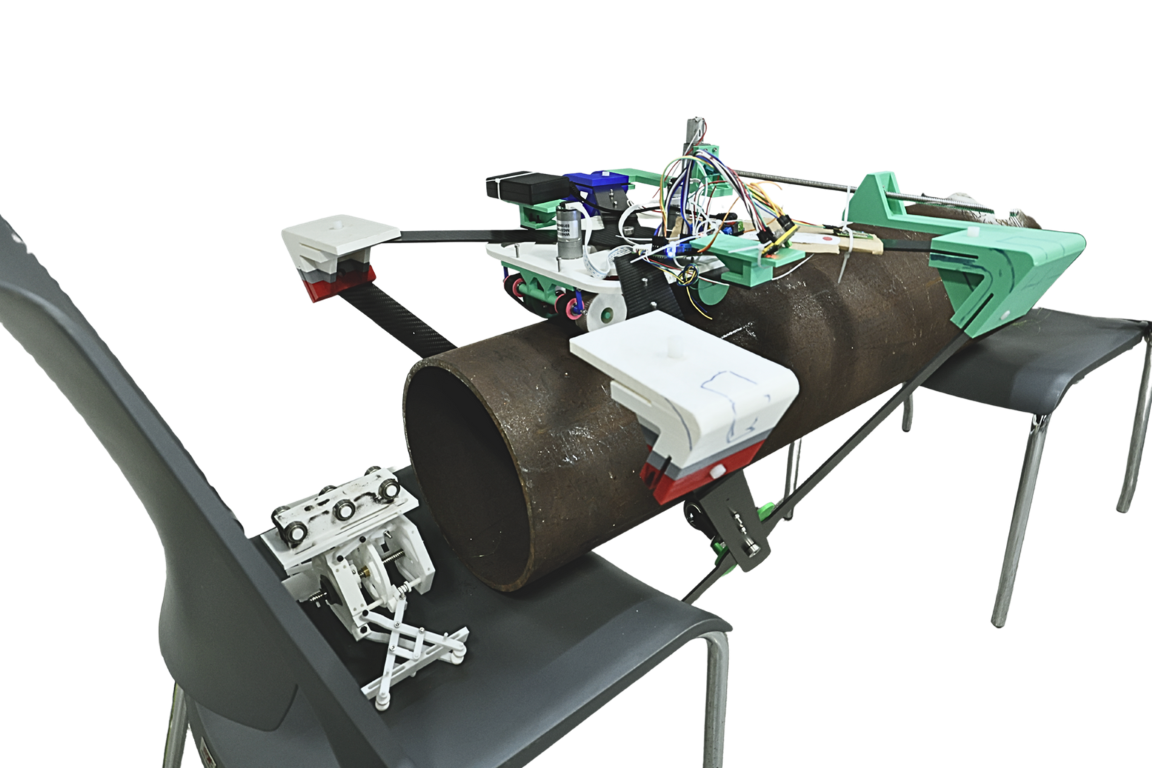
\includegraphics[width=0.6\textwidth]{Pasted image 20250814141635.png}
     \caption{管外机器人实物}
     
   
    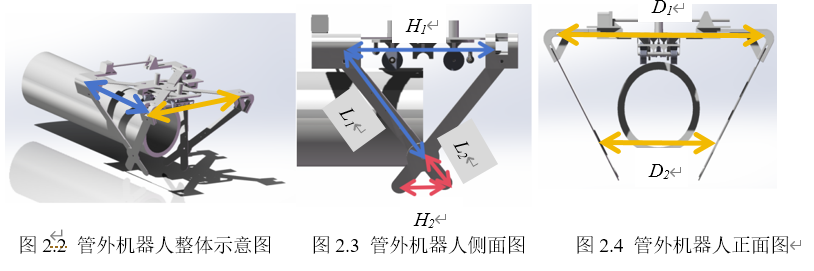
\includegraphics[width=1\textwidth]{Pasted image 20250814134613.png}
    \caption{立体叉字伸缩结构示意图}
     
\end{figure}

\begin{figure}[htbp]
    \centering
    \begin{subfigure}{0.45\textwidth}
        \centering
        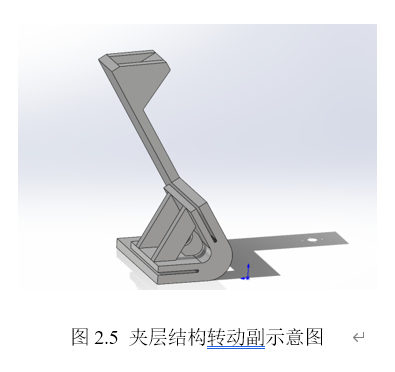
\includegraphics[width=\textwidth]{Pasted image 20250814134739.png}
        \caption{转动副结构示意图}
        
    \end{subfigure}
    \hfill
    \begin{subfigure}{0.45\textwidth}
        \centering
        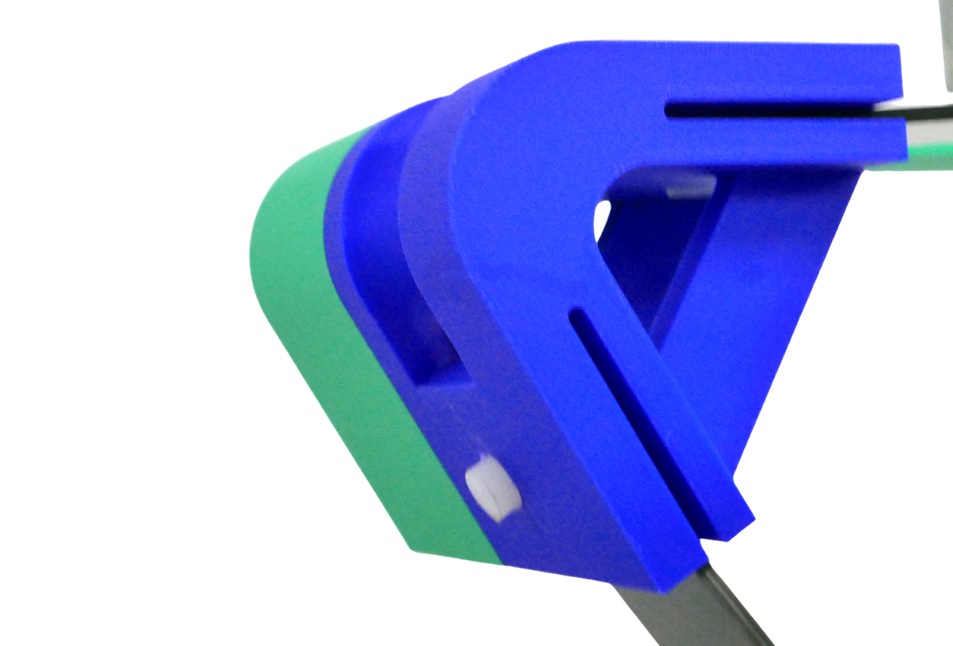
\includegraphics[width=\textwidth]{Pasted image 20250814141702.png}
        \caption{转动副实物图}
    \end{subfigure}
    \caption{三明治夹层转动副设计}
\end{figure}





\begin{figure}[htbp]
    \subsubsection{管内机器人设计}
    管内机器人采用"X形剪刀结构"，搭载海尔贝克磁铁阵列，可在不增加磁铁用量的前提下显著提升吸附力，同时减少轭部厚度，降低整体重量，提高机器人的动态响应能力。
    \centering
    \begin{subfigure}{0.45\textwidth}
        \centering
        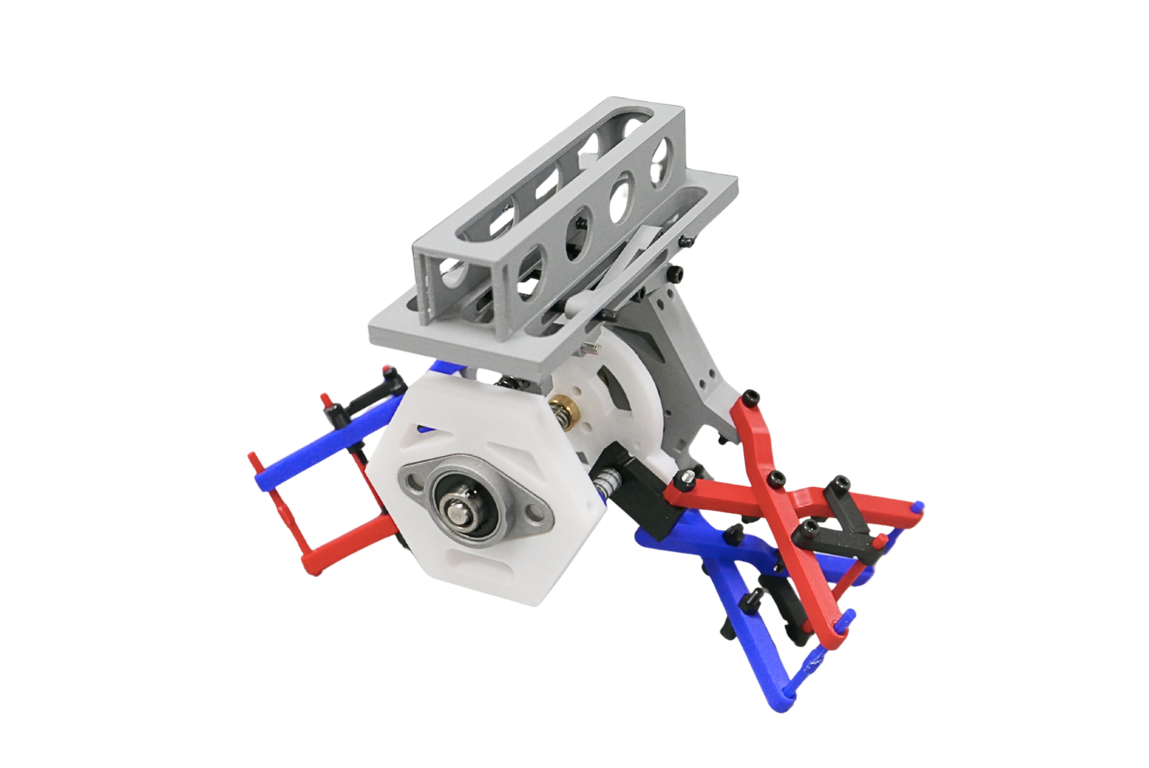
\includegraphics[width=\textwidth]{Pasted image 20250814144851.png}
        \caption{管内机器人整体设计}
        
    \end{subfigure}
    \hfill
    \begin{subfigure}{0.45\textwidth}
        \centering
        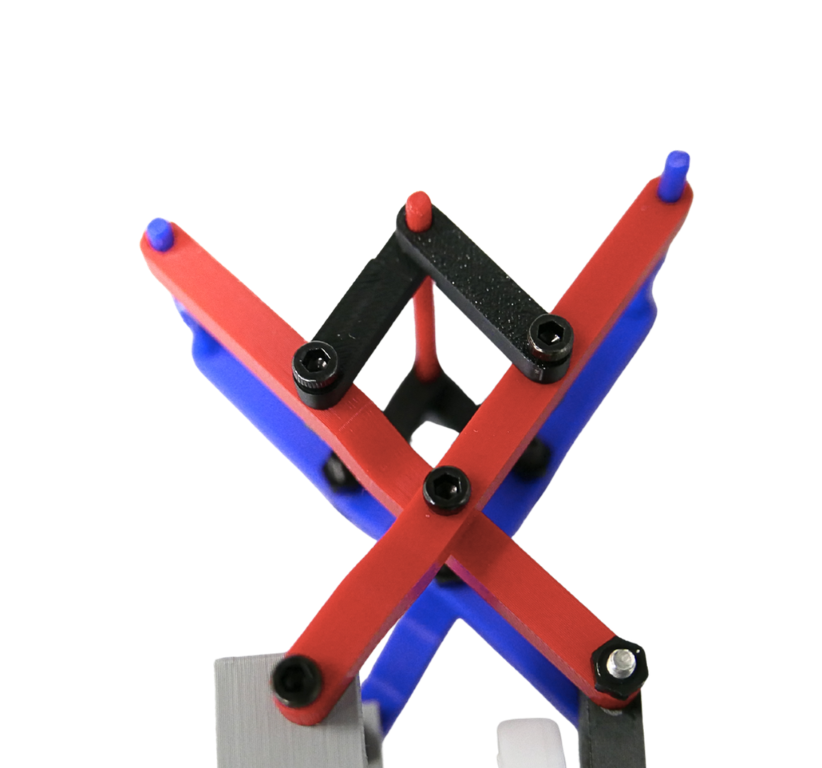
\includegraphics[width=\textwidth]{Pasted image 20250814144833.png}
        \caption{X形剪刀结构}
    \end{subfigure}
    
\end{figure}




\begin{figure}[htbp]
    \subsubsection{磁吸机构设计}
    由于相邻磁铁的N极与S极相互吸引，未固定的磁铁易翻转贴合，导致阵列失效。为解决上述问题，本项目设计了一种自锁管约束装置。自锁管为根据磁铁尺寸定制的管道结构，通过上下左右的物理限位，阻止磁铁在装配过程中翻转。磁铁按预设角度依次滑入管道，强制形成目标阵列排布。

    \centering
    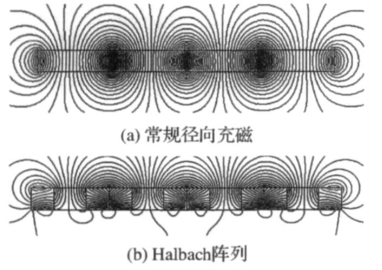
\includegraphics[width=0.6\textwidth]{Pasted image 20250730171808.png}
    \caption{自锁管约束装置}
\end{figure}

\begin{figure}[htbp]
    \centering
    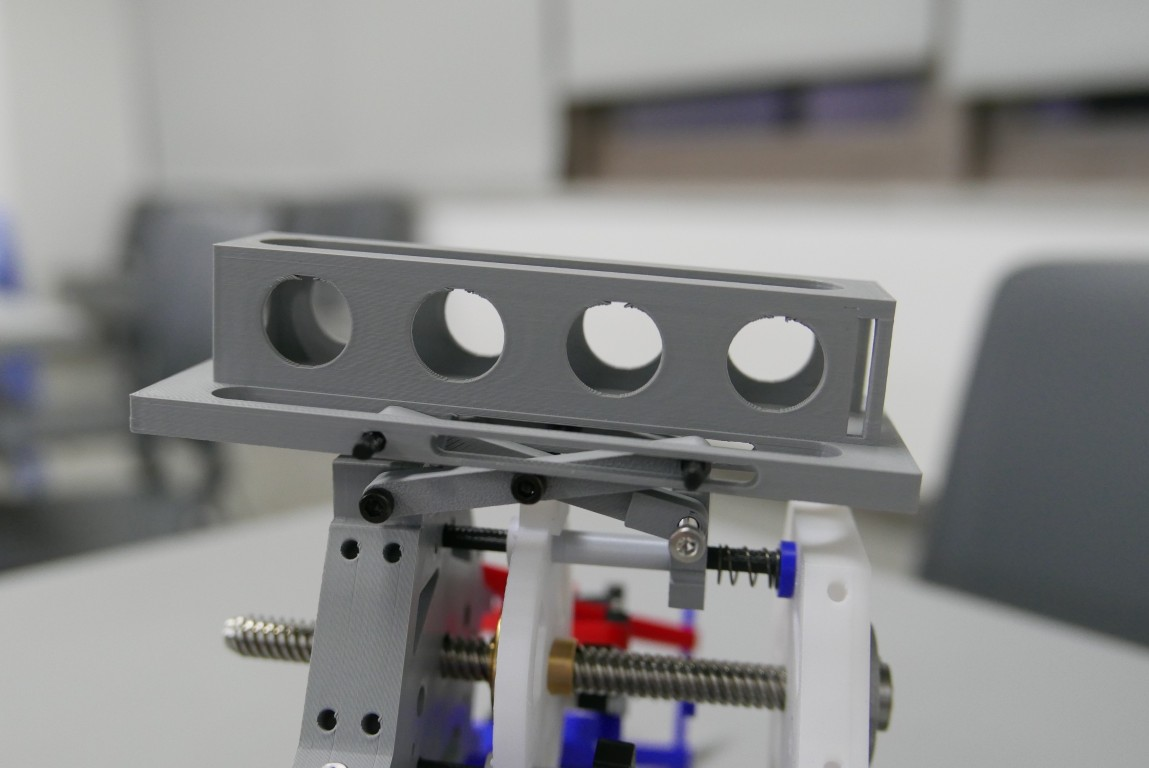
\includegraphics[width=0.6\textwidth]{1030761.jpg}
    \caption{海尔贝克阵列实物}
\end{figure}

\newpage
\subsection{超声波通讯}

\subsubsection{概述}

管外机器人与管内机器人（以下统称为管道机器人）之间的通讯非常困难。

管道机器人作业的管道为金属材质，不仅对磁感线有强干扰作用，也对电磁信号具有\textbf{强屏蔽作用}和\textbf{强反射作用}。这意味着，若管道机器人之间的通讯采用电磁信号，其传播过程中不仅会受到管道的强屏蔽，而且会受到自身反射信号的干扰。

为了尽量减少管道对于通信的影响，增强机器人的通信能力及鲁棒性，我们决定从三个方向入手：

\begin{itemize}
    \item 降低管道机器人之间的通信需求和通信流量密度，降低通信能耗和通信次数，以降低干扰的影响；
    \item 更改管道机器人之间的通讯信号载体，选用抗干扰性更强的信号；
    \item 增加扩频解扩、滤波等一系列手段，尽可能排除干扰信号、杂波信号与反射信号的影响。
\end{itemize}

上述三个方向的具体技术细节将在下文详细展开。

\subsubsection{方向1：降低通信需求}

此方向解决了两个问题：

\begin{itemize}
    \item 管道内通信干扰大，若通讯信息密度大，则传达信息不稳定，不可持续；
    \item 管道狭窄、危险，机器人对于功耗的要求高，若通信信息密度大，则能耗可能过高，不可持续；
\end{itemize}

具体来说，我们的管道机器人之间的相互通信仅\textbf{收发简单、稳健性强的二进制编码}以应对回声、障碍物造成的信号混叠与衰减。为了减少二进制编码传输效率低的影响，我们给管内机器人配备了\textbf{边缘计算能力}，通过增加管内计算降低通信流量密度。具体做法为，在管内机器人的香橙派上部署视觉模型，对管内检测到的"管道轻微损伤、管道严重损伤、需进一步勘察"等状况进行识别分类，每一类别对应唯一的二进制编码，管内仅需向管外发送二进制编码。 

此方案优势在于设备体积小，功耗低，在同等电池容量情况下能够提高管内机器人的续航，减少管内机器人因低电量无法返回管外的状况发生。同时，通信需求低也降低了管内复杂环境对于通信的干扰。

\subsubsection{方向2：更改通讯信号载体}

\paragraph{超声波信号通讯}

面对管道内强烈的电磁干扰与屏蔽，我们决定采用波长短、功率低的超声波信号进行通讯。在电磁干扰复杂的环境下，如在存在强电磁场或无线电干扰的场所，超声波作为一种机械波，其传播相对稳定，\textbf{不会受到电磁干扰}，从而保证了通信的可靠性。同时，其短波长使得超声波的方向性更强，在相同的环境中，其遇到的障碍物相对尺寸与波长的比值可能较小，因此绕射能力较弱，传播方向性较强。这意味着超声波在传播过程中，其能量相对集中在主传播方向上，遇到障碍物时，\textbf{反射波的能量相对较弱}，对入射波的影响相对较小。

\subsubsection{方向3：增加扩频和滤波}

\paragraph{Gold序列的生成原理和性质}

在介绍Gold序列前需要先介绍$m$序列。
$m$序列是最常见的PN（$Pseudo-Noise$，伪随机）序列，它的一种生成方式是对$N$位二进制数的末尾两位异或并将结果移至第一位，其余位逻辑右移。对某个$N$位二进制序列不断进行该过程可得到周期$2^N-1$的$N$阶$m$序列。
Gold序列正是由优选$m$序列对生成。
两个$m$序列$m_1(n)、m_2(n)$如果满足：

\begin{enumerate}
    \item 阶数相同
    \item 存在整数$0\leq\tau\leq2^n-1$，满足$|R_{12}(\tau)|\le2^{\frac{n+1}{2}}+1(n=2k+1,k\in N)$
\end{enumerate}

则这两个序列就构成优选$m$序列对。
优选序列对之异或构成一个Gold序列，$G(t)=m_1(n)\oplus m_2(n+\tau)$就是一个$Gold$序列。

Gold序列具有优良的\textbf{强自相关性}和\textbf{弱互相关性}，这对于下文中的扩频、加密操作具有重要意义。

\begin{tcolorbox}[title=数字序列的相关性]
数字序列的相关性指不同数字序列的相似程度。
计算方法如下：
两个数字序列转化成双极性序列，即$\{0,1\}$映射为$\{-1,+1\}$。然后二者做按位积，得到的新序列之后再调用互相关函数进行滑动相乘并求和。
互相关函数（CCF）：衡量两个序列$x(n)$ 和$y(n)$在不同时移 $\tau$下的相似性，定义为：
$$R_{x y}(\tau)=\sum_{n=0}^{N-1} x(n) \cdot y(n+\tau)$$
其中$x(n), y(n) \in\{-1,+1\}$ (二进制$0$映射为$-1$，$1$映射为$+1$)。
\end{tcolorbox}

\paragraph{DSSS扩频}

\textbf{DSSS扩频}指使用窄宽度$PN$数字序列（$Pseudo-Noise$，伪随机）对\textbf{待发送的原始比特流}进行处理的操作。我们采用Gold序列作为扩频用序列$p(n)$，将管内机器人对管道内勘测状况分类得到的二进制编码作为原始比特流$r(n)$，发射端实际发射信号为$r(n)\oplus p(n)$。

接收端进行解扩操作，利用Gold序列$p(n)$的\textbf{强自相关性}。因而有$r(n)\oplus p(n)\oplus p(n)=r(n)$。则接收方解调得到$r(n)\oplus p(n)$数字信号后，对该数字信号异或$p(n)$即可得到原始比特流$r(n)$。此处的异或也可以理解为将比特流转化成双极性序列后的算术乘法。

同时，Gold序列$p(n)$的\textbf{弱互相关性}使得Gold序列$p(t)$很容易与自身的时移序列$p(t+\tau)$分离出来，也容易与其他伪随机序列分离出来。这一性质保证扩频操作能实现抗干扰、加密和多通道通讯。这是因为Gold序列互相关性低有\textbf{两层含义}：Gold序列$p(t)$和其他伪随机序列相关性低；Gold序列$p(t)$与自身的移位序列$p(t+\tau)$的相关性也很低。

扩频与解扩的处理有\textbf{三个好处}：

\begin{enumerate}
    \item 能够提高信号的抗干扰性。扩频让干扰信息与有用信息的能量均被"稀释"，而有用信息的能量在解扩时会重新聚集。
    \item $p(n)$序列伪随机且对第三方不透明，使得扩频后的信号对第三方而言类似白噪声。因而$p(n)$可以对$r(n)$进行加密，$r(n)\oplus p(n)$即为密文，通讯信息不易泄露。
    \item 采用\textbf{弱互相关性}的$Gold$序列生成$p(n)$。$p_1(n)$、$p_2(n)$等多个伪随机序列在实现加密的同时可以实现低干扰的多通道通讯，允许多机器人同时工作。
\end{enumerate}

\paragraph{滑动匹配法同步}

Gold序列的弱相关性同时也意味着$$p(n)\oplus p(n+\tau)\neq1$$所以，考虑到信号传递频繁折射发射导致的时移，在正式解扩前，接收端与发射端需要进行同步。
我们采用\textbf{滑动匹配法}进行同步。滑动匹配法的算法如下：

\begin{enumerate}
    \item 本地PN序列以固定步长（如$\frac{1}{2} \text{Chip}$）滑动，与接收到信号进行相关性运算。当计算得相关性高于某阈值时判定捕获成功。
    \item 为了\textbf{进一步增强}该同步机制，在原始比特流中加入事先约定好的同步口令，在接收端不断进行$Gold$序列滑动。
    \item 若能在某个滑动值下相关性高于阈值，并且还原出该口令，则认为同步完成。
\end{enumerate}

\begin{table}[htbp]
\centering
\caption{不同解调法对比}
\begin{tabular}{p{0.3\textwidth}p{0.25\textwidth}p{0.2\textwidth}p{0.2\textwidth}}
\toprule
\textbf{解调法} & \textbf{是否需要载波同步} & \textbf{抗多径能力} & \textbf{实现复杂度} \\
\midrule
直接相位判决法 & 需要 & 差 & 较高 \\
滑动匹配法 & 不需要 & 强 & 简洁 \\
\bottomrule
\end{tabular}
\end{table}

\paragraph{多机器人并行工作}

使用扩频的方法同时还可以减少相同通讯系统之间的相互干扰，满足需要多套管道机器人同时作业的需求。原理如下：

假设某时刻管内机器人1,2与管外机器人一起工作。管外机器人对接收到的超声波信号进行解调，得到Gold序列扩频后的信号$t_1(n)、t_2(n)$。其中$t_1(n)=r_1(n)\oplus p_1(n)$，$t_2(n)=r_2(n)\oplus p_2(n)$，$r_1(n)$为管内机器人1的原始比特流，$p_1(n)$为Gold序列1。对管内机器人2同理。

由$Gold$序列的\textbf{强自相关性}，解扩过程实际处理如下
$$t_i(n)\oplus p_i(n)=r_i(n)\oplus p_i(n)\oplus p_i(n)=r_i(n)，i=0,1$$
于是管外机器人成功得到管内机器人发送的有效数据。

由$Gold$序列的\textbf{弱互相关性}
$$ t_i(n)\oplus p_j(n)\neq r_i(n),i\neq j $$$$ t_i(n)\oplus p_j(n)=r_i(n)\oplus (p_i(n)\oplus p_j(n))\approx 0,i\neq j$$
因此管内机器人1,2可以同时工作，各自独立与管外机器人通讯，互不干扰。

同时作业的机器人数量可以进一步增加。

\paragraph{积分滤波}

即使经过上述一系列的操作，对接收信号进行解调、解扩后得到数字信号，最终得到的比特流依然可能蕴含噪声、毛刺。

我们对每周期进行积分，从而确定该周期传递的信息，提升信噪比。

积分滤波是一种信号处理技术，主要用于对信号进行平滑和低通滤波。它通过对输入信号进行积分运算，去除高频噪声和干扰，提取信号的低频成分。积分滤波通过对信号进行积分运算，可以有效地平滑信号，去除高频噪声和干扰。这是因为积分运算可以对信号中的高频成分进行衰减，而对低频成分的影响较小。积分滤波相当于一个低通滤波器，其频率响应在低频段具有较高的增益，而在高频段逐渐衰减。因此，它可以有效地滤除信号中的高频成分，保留低频成分。

\subsubsection{总结}

上述流程可总结为：

\begin{quote}
原始比特流 $\rightarrow$ 扩频 $\rightarrow$ 调制 $\rightarrow$ 解调 $\rightarrow$ 解扩 $\rightarrow$ 原始比特流
\end{quote}

\begin{tcolorbox}[title=发送端]
\begin{enumerate}
    \item 在MCU中，原始比特流$r(n)$首先和$\text{Gold}(n)$进行异或操作，完成扩频；
    \item 扩频后的数字信号通过相位映射把信息加载到待发送的$\cos\varphi_k$的相位差中，完成调制；
    \item 最终该模拟信号经过放大后发射。
\end{enumerate}
\end{tcolorbox}

\begin{tcolorbox}[title=接收端]
\begin{enumerate}
    \item 接收电路接收到$\cos(\varphi_k)$，对$\cos(\varphi_k)$进行相位偏移得到$\sin(\varphi_k)$；
    \item $\cos(\varphi_k)$与$\cos(\varphi_k)$分别进入ADC1与ADC2，在复数域运算解得相位$\varphi_k$；
    \item 计算$\Delta\varphi_k=\varphi_k-\varphi_{k-1}$，完成相位逆映射，得到数字信号；
    \item 在$MCU$中数字信号和$\text{Gold}(n+\tau)$异或，完成解扩，最终得到原始比特流$r(n)$。
\end{enumerate}
\end{tcolorbox}

上述流程尽最大可能排除了管道内的电磁干扰、杂波干扰和反射干扰，具有低功耗、高鲁棒性和高效率的特点。

\subsection{无线充电模块}

\subsubsection{为什么决定设计无线充电装置？}

\paragraph{磁牵引管道机器人困境}

管道外机器人在管道外作业时，不仅需要实时变径转动，适应管道外侧的法兰盘与支架得以通过，还需要借助海姆贝克阵列铷磁铁实现对管内机器人的牵引，以及对管内机器人外传的超声波讯息进行解调编码，以上的一系列操作都使得管外机器人的功耗难以降低，无法实现长距离的牵引工作。

为了解决如上的大功耗续航短问题，我们团队首先从降低功耗这一角度出发，优化了机器人机构，减重了机器人重量，并采用更高效的电机驱动，使机器人整体功耗降低，但续航时间依然无法满足实际需求。

因此，一个为机器人在运行过程中充电的想法应运而生。

\paragraph{无线充电的具体使用场景介绍}

为了既能实现能量补充，又能减少人力物力财力，我们决定设计一款部署简单、能量传输功率大、安全系数高的无线充电接收、发射模块与基站。

我们希望这款无线充电装置能够应用于磁牵引管道机器人，实现机器人运行过程中的能量补充，延长机器人的运行时间，降低维护成本，提高工作效率。

\subsubsection{无线充电装置的设计要点}

无线充电装置的设计必须满足《无线充电（电力传输）设备无线电管理暂行规定》中对\textbf{发射频率}、\textbf{充电功率}等关键参数的要求，以及新规则中对\textbf{尺寸}的要求。

\paragraph{优越特性}

\begin{itemize}
    \item \textbf{安全性高与智能控制:}
    \begin{itemize}
        \item 具有过流保护、过温保护、\textbf{异物检测}等保护措施。
        \item 配合接收端可实现\textbf{恒功率充电}。
        \item 能够实现\textbf{识别到管外机器人上的接收线圈后才开始充电}，具有良好的安全性。
        \item 接收端即使在单片机程序跑飞的情况下，也能通过模拟控制维持恒流充电，\textbf{安全系数较高}。
        \item 系统具备异物检测功能，可防止为接收线圈之外的物品辐射能量。
    \end{itemize}
    \item \textbf{硬件优势:}
    \begin{itemize}
        \item 发射端的PCB尺寸仅为 $53\text{mm} \times 41\text{mm}$，\textbf{非常小巧}。
        \item 工作时温升较低，\textbf{无需主动散热}，可随意放置。
        \item 发射端静态功耗小于 $1\text{W}$。
    \end{itemize}
\end{itemize}

\paragraph{关键参数展示}

\begin{itemize}
    \item \textbf{工作频率:} $148\text{KHz}$。
    \item \textbf{能量交互面尺寸:} 约 $90\text{mm} \times 90\text{mm}$。
    \item \textbf{最高持续输出功率:} 设计目标是在线圈相距 $2\text{cm}$ 以内时，最大充电功率大于 $120\text{W}$。
\end{itemize}

\begin{table}[htbp]
\centering
\caption{无线充电装置性能测试}
\begin{tabular}{p{0.3\textwidth}p{0.6\textwidth}}
\toprule
\textbf{项目} & \textbf{测试效果} \\
\midrule
\textbf{充电时间} & 实测显示，该装置约 $40$ 秒即可将3S锂电池从零充至满电。充电时通过缓启动机制提高系统稳定性。 \\
\textbf{充电效率} & 该系统在 $120\text{W}$ 负载下，发射端热点温度仅 $40^\circ\text{C}$ 左右，表明\textbf{散热表现优秀}。接收端通过PID控制输出电流实现充电功率闭环，静态误差小于 $0.2\text{W}$。最终可实现接近45\%的充电效率。 \\
\textbf{充电传输范围} & 设计目标是在线圈\textbf{相距 $2\text{cm}$ 以内}时，最大充电功率大于 $120\text{W}$。 \\
\textbf{应用后扩大的作业半径} & 充满电后，经功耗仿真、理论计算，预估管外机器人续航提升至\textbf{10km} \\
\bottomrule
\end{tabular}
\end{table}

\subsubsection{硬件电路设计展示}

\paragraph{发射端电路设计}

发射端设计 (LC 谐振)

\begin{itemize}
    \item \textbf{拓扑与激励:} 采用四颗功率 MOSFET 构成\textbf{全桥拓扑}。发射线圈采用 \textbf{LC 补偿}。全桥电路将 $24\text{V}$ 直流输入转换为高频交流信号，驱动 $\text{LC}$ 谐振线圈。
    \item \textbf{主控与驱动:} $\text{STM}32\text{F}334$ 利用内部的 $\text{HRTIM}$ 进行精准的\textbf{调频控制}。栅极驱动电路采用了 $\text{MP}18024$ 高低侧驱动器。
\end{itemize}

\begin{figure}[htbp]
    \centering
    \begin{subfigure}{0.3\textwidth}
        \centering
        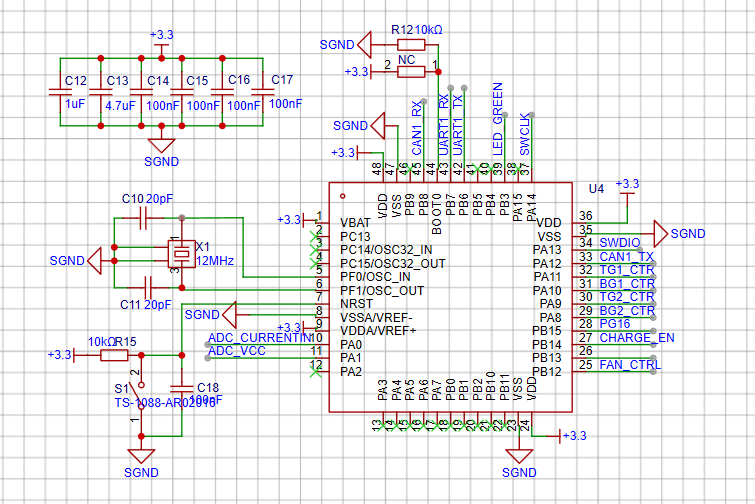
\includegraphics[width=\textwidth]{image.png}
        \caption{主控}
    \end{subfigure}
    \hfill
    \begin{subfigure}{0.3\textwidth}
        \centering
        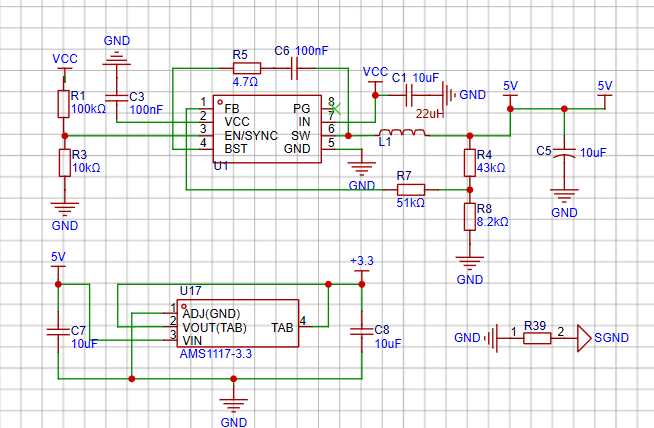
\includegraphics[width=\textwidth]{image-1.png}
        \caption{主控电源回路}
    \end{subfigure}
    \hfill
    \begin{subfigure}{0.3\textwidth}
        \centering
        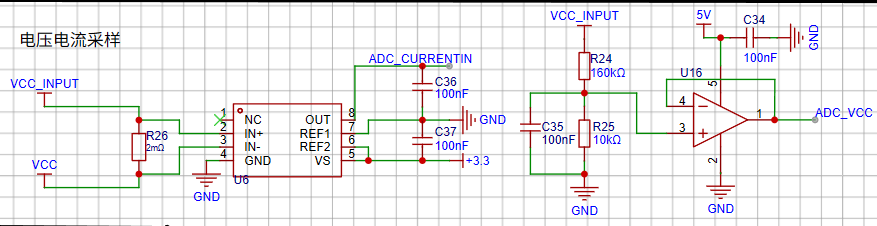
\includegraphics[width=\textwidth]{image-8.png}
        \caption{采样电路}
    \end{subfigure}
    
    \begin{subfigure}{0.3\textwidth}
        \centering
        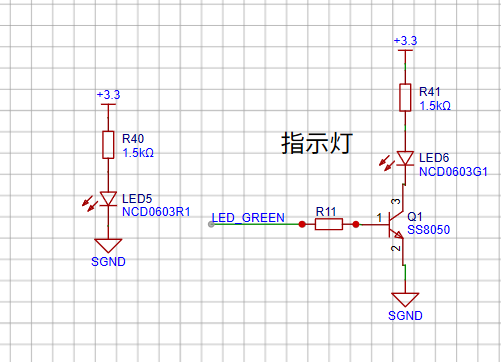
\includegraphics[width=\textwidth]{image-2.png}
        \caption{工作指示灯}
    \end{subfigure}
    \hfill
    \begin{subfigure}{0.3\textwidth}
        \centering
        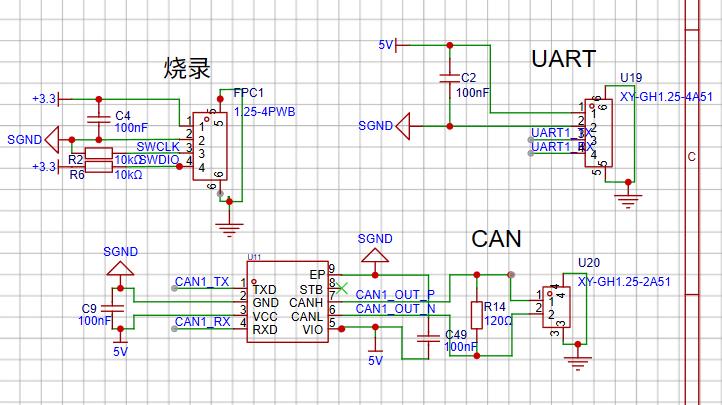
\includegraphics[width=\textwidth]{image-3.png}
        \caption{通信接口}
    \end{subfigure}
    \hfill
    \begin{subfigure}{0.3\textwidth}
        \centering
        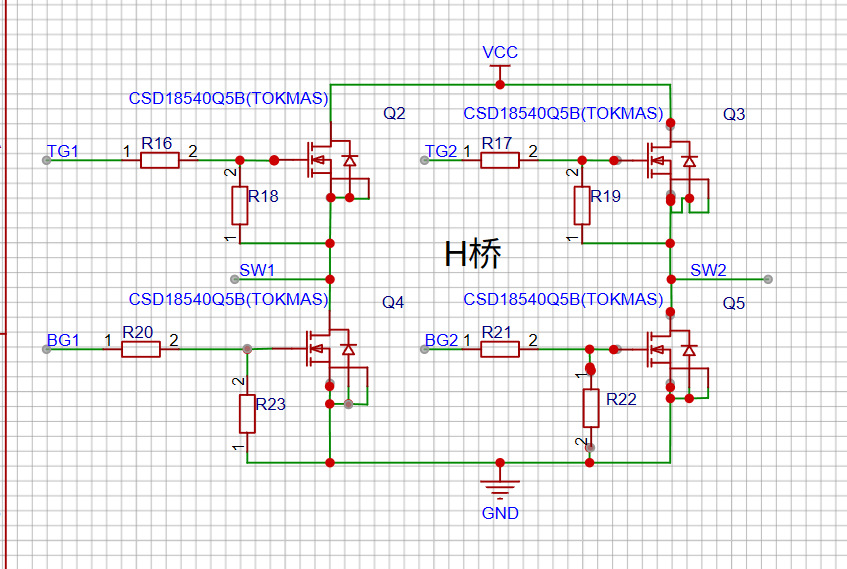
\includegraphics[width=\textwidth]{image-4.png}
        \caption{H桥电路}
    \end{subfigure}
    
    \begin{subfigure}{0.45\textwidth}
        \centering
        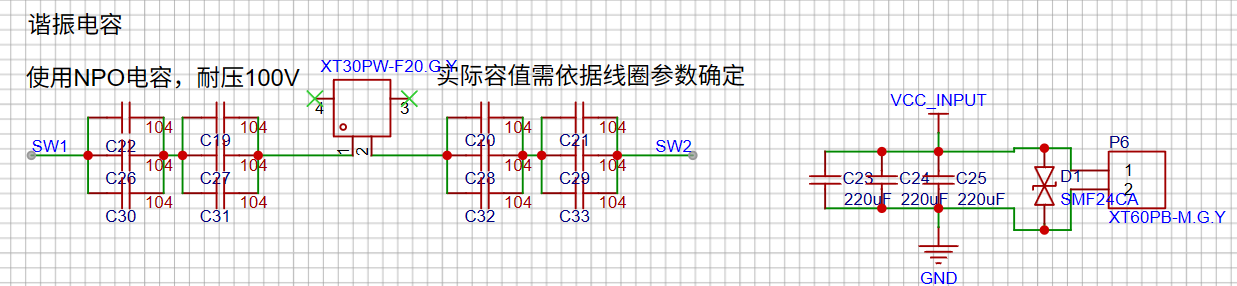
\includegraphics[width=\textwidth]{image-6.png}
        \caption{LC谐振回路}
    \end{subfigure}
    \hfill
    \begin{subfigure}{0.45\textwidth}
        \centering
        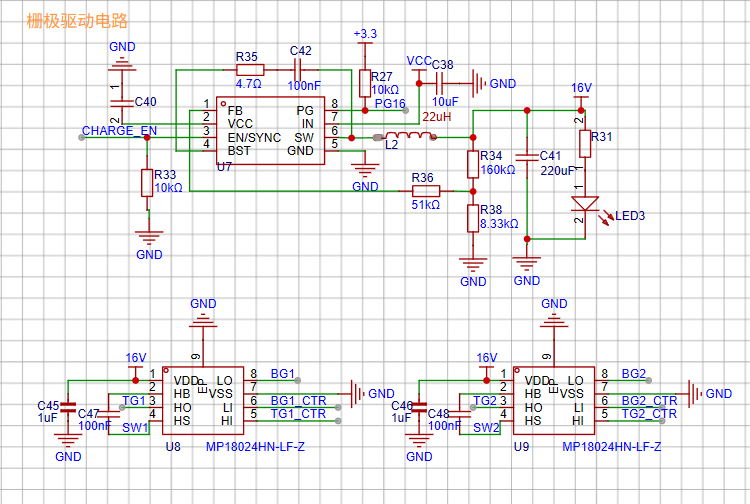
\includegraphics[width=\textwidth]{image-7.png}
        \caption{H桥驱动电源回路}
    \end{subfigure}
    \caption{发射端电路设计}
\end{figure}

\paragraph{接收端电路设计}

接收端设计 (LCC 谐振与 Buck-Boost)

\begin{itemize}
    \item \textbf{拓扑优化:} 为解决发射端方波中的高次谐波问题（特别是三次谐波），接收线圈的补偿网络由 $\text{LC}$ 修改为 \textbf{LCC 补偿}，额外并联了一个高频滤波电容 $\text{Cf}$，以抑制高次谐波。
    \item \textbf{DC-DC 变换:} 接收端使用了整流滤波 $+$ 电流模式 $\text{DCDC}$ 的设计。选用 \textbf{Buck-Boost 电路}（控制器为 $\text{LT}3790\text{EFE}$）以应对接收端感应电压在 $10\text{V}$ 到 $50\text{V}$ 之间波动的情况。
    \item \textbf{控制方式:} $\text{LT}3790\text{EFE}$ 具备\textbf{恒流模式}。$\text{STM}32\text{F}334$ 通过 $\text{INA}226$ 监测电容充电功率，通过 \textbf{PID 算法}实现充电功率闭环。
\end{itemize}

\begin{figure}[htbp]
    \centering
    \begin{subfigure}{0.3\textwidth}
        \centering
        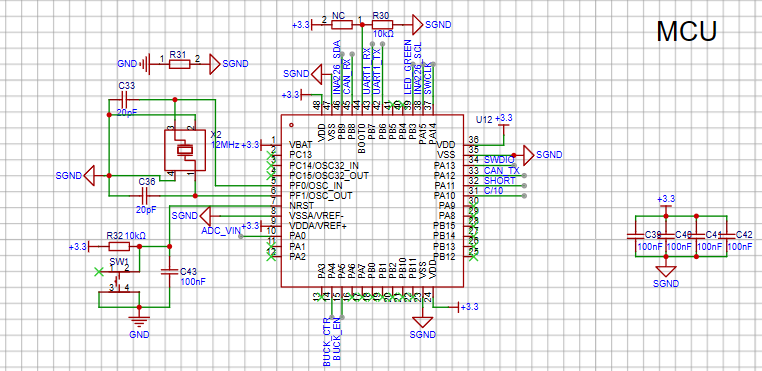
\includegraphics[width=\textwidth]{image-15.png}
        \caption{主控}
    \end{subfigure}
    \hfill
    \begin{subfigure}{0.3\textwidth}
        \centering
        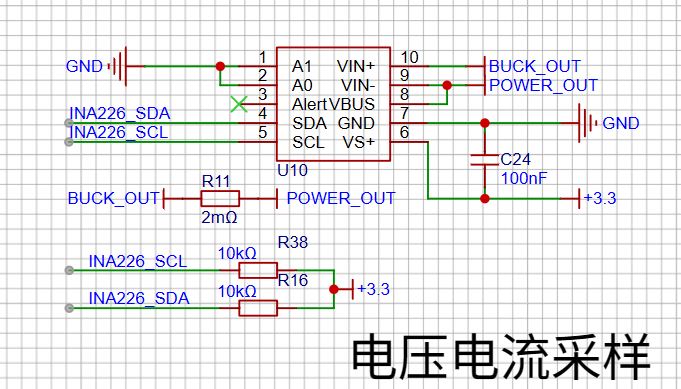
\includegraphics[width=\textwidth]{image-18.png}
        \caption{主控采样}
    \end{subfigure}
    \hfill
    \begin{subfigure}{0.3\textwidth}
        \centering
        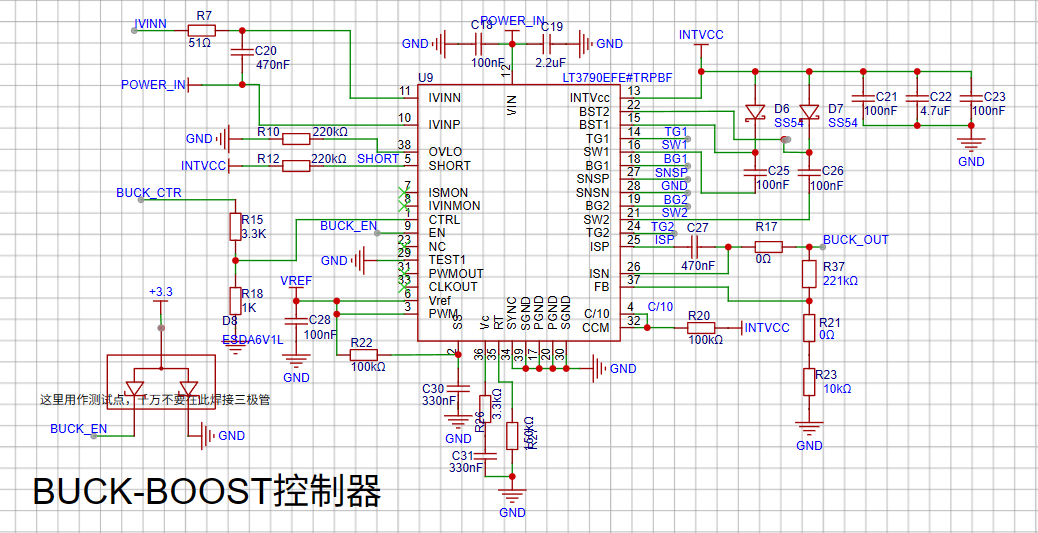
\includegraphics[width=\textwidth]{image-14.png}
        \caption{LT3790EFE电路}
    \end{subfigure}
    
    \begin{subfigure}{0.45\textwidth}
        \centering
        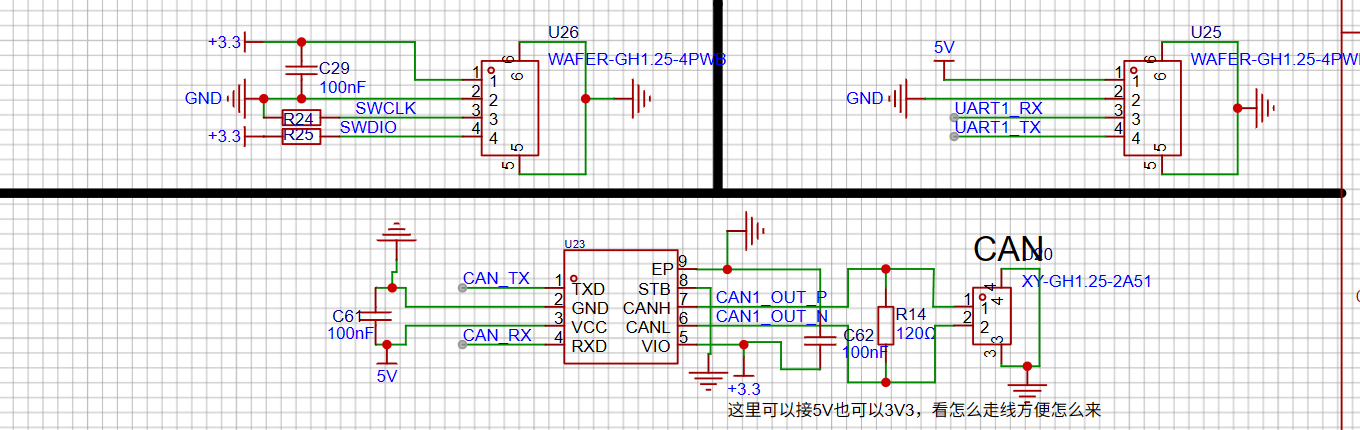
\includegraphics[width=\textwidth]{image-16.png}
        \caption{通讯、烧录接口}
    \end{subfigure}
    \hfill
    \begin{subfigure}{0.45\textwidth}
        \centering
        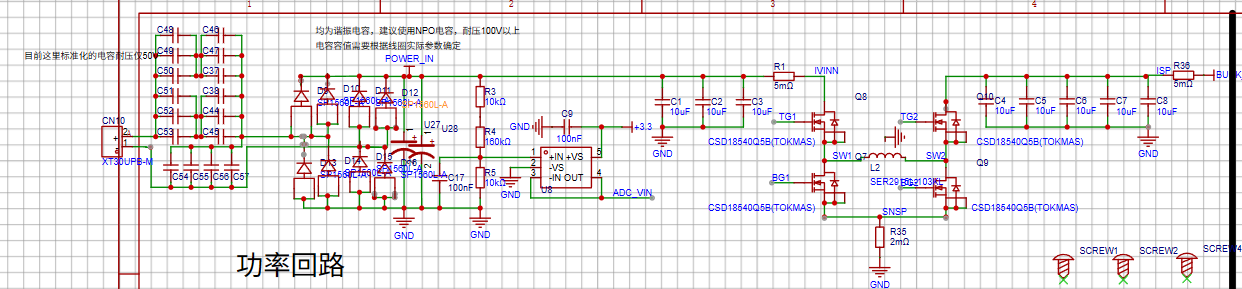
\includegraphics[width=\textwidth]{image-17.png}
        \caption{功率回路}
    \end{subfigure}
    \caption{接收端电路设计}
\end{figure}

\subsubsection{异物检测与线圈识别原理}

\begin{itemize}
    \item \textbf{机制:} 采用类似 $\text{Q}$ 值检测的思路，通过采集发射端输入电流的\textbf{直流成分}（"铁损"）来实现异物检测和线圈识别。
    \item \textbf{异物检测:} 当金属异物靠近线圈时，交变电磁场在金属中产生涡流，涡流产热功率远大于环境中的"铁损"，导致采集到的输入电流\textbf{显著增大}。
    \item \textbf{线圈识别:} 接收线圈靠近时，由于线圈背面的隔磁片作用，空间中泄露的电磁波急剧减少，\textbf{铁损值降低}，输入电流显著下降。通过设置电流阈值，即可区分无物品、有异物和有接收线圈三种状态。
\end{itemize}

\begin{figure}[htbp]
\subsubsection{部分仿真展示}


    \centering
    \begin{subfigure}{0.3\textwidth}
        \centering
        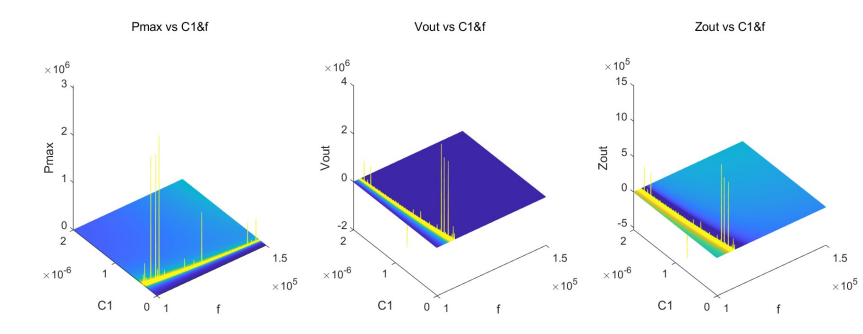
\includegraphics[width=\textwidth]{image-10.png}
        \caption{谐振电容选型}
    \end{subfigure}
    \hfill
    \begin{subfigure}{0.3\textwidth}
        \centering
        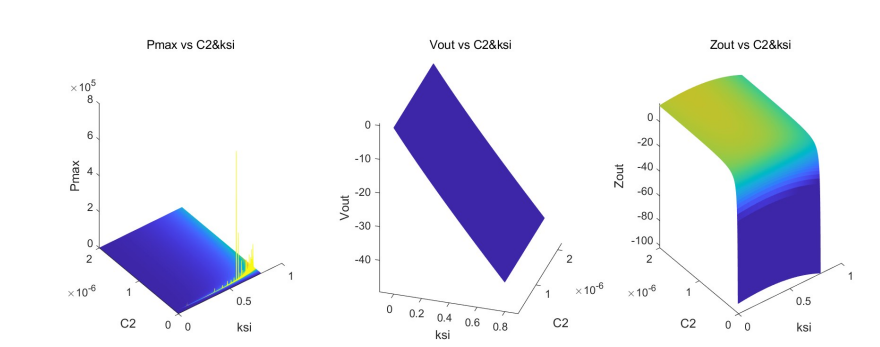
\includegraphics[width=\textwidth]{image-11.png}
        \caption{耦合系数扫描}
    \end{subfigure}
    \hfill
    \begin{subfigure}{0.3\textwidth}
        \centering
        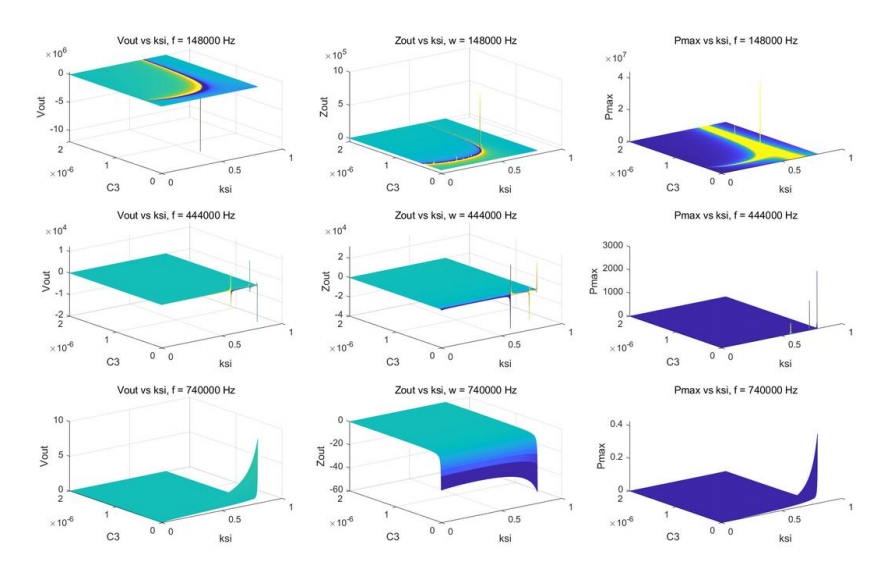
\includegraphics[width=\textwidth]{image-12.png}
        \caption{高频滤波电容选型}
    \end{subfigure}
    \caption{无线充电系统仿真}
\end{figure}


\begin{figure}[htbp]
\subsubsection{实物展示}


    \centering
    \begin{subfigure}{0.3\textwidth}
        \centering
        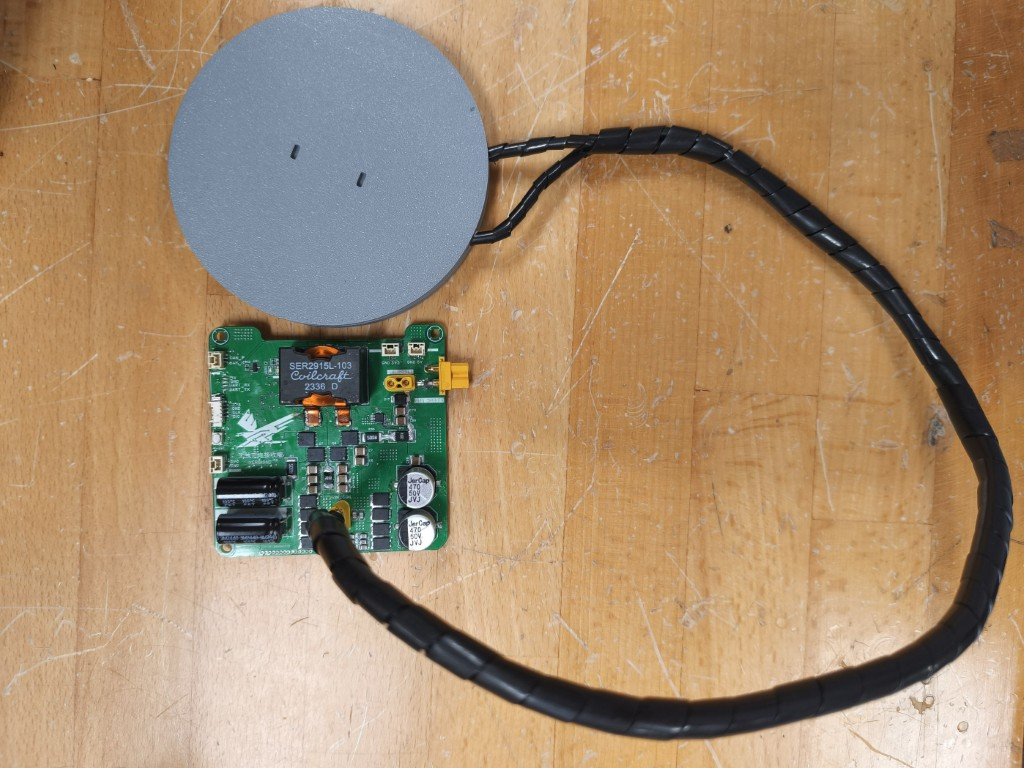
\includegraphics[width=\textwidth]{3cfc33965f3158fdb45d643b2d1006fc.png}
    \end{subfigure}
    \hfill
    \begin{subfigure}{0.3\textwidth}
        \centering
        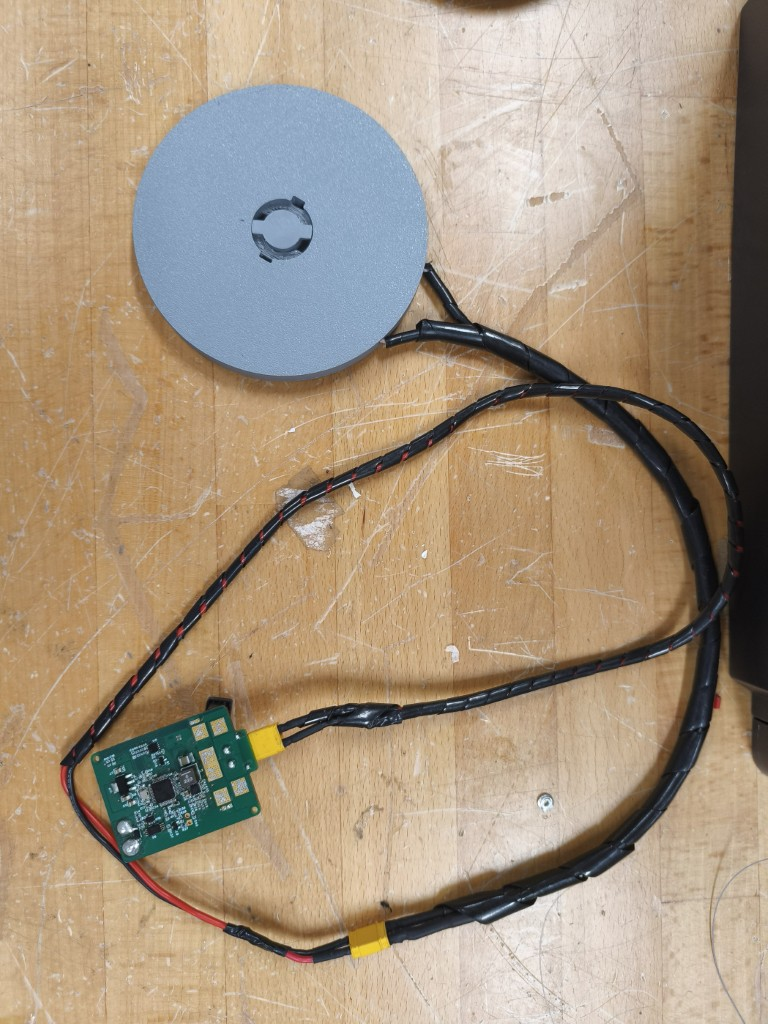
\includegraphics[width=\textwidth]{7f2163c3e6e607294780f668e07b28c0.png}
    \end{subfigure}
    \hfill
    \begin{subfigure}{0.3\textwidth}
        \centering
        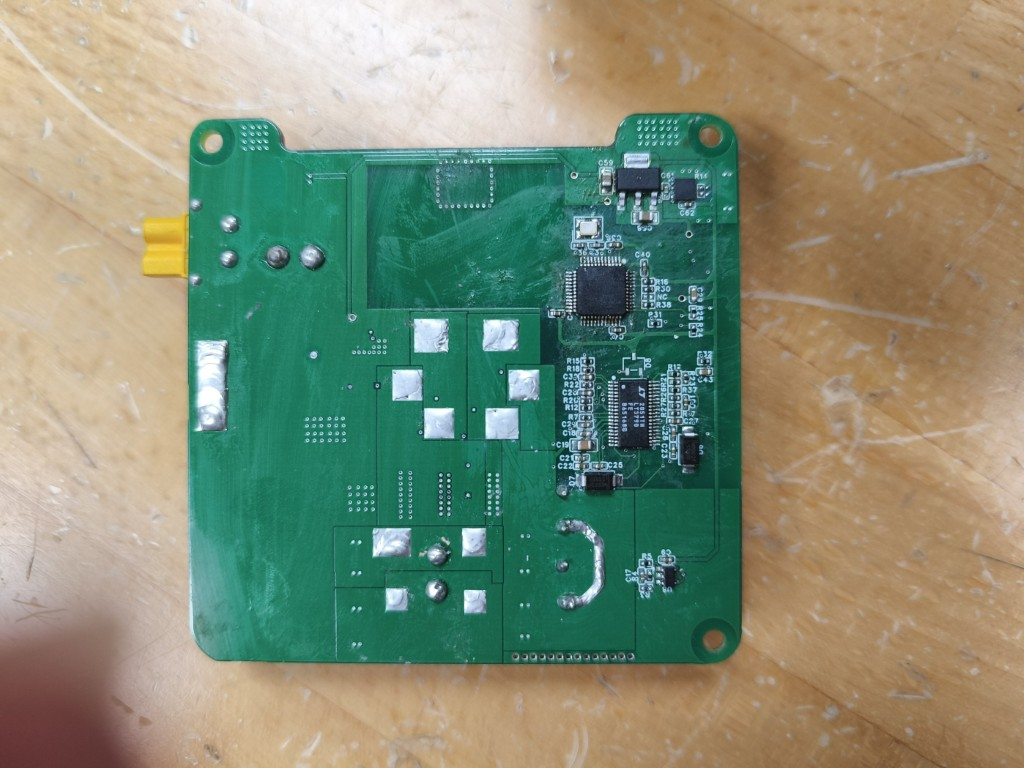
\includegraphics[width=\textwidth]{b45033fc59faf143cb6a99340f6c8112.png}
    \end{subfigure}
    \caption{无线充电装置实物}
\end{figure}





\section{市场分析}

\subsection{行业现状与核心痛点}

工业管道作为能源传输、化工生产、污水排放等领域的核心基础设施，其运行状态直接关系到企业生产安全与生态环境可持续性。当前我国工业管道环境治理领域面临三大核心现状，痛点突出且亟待解决：



\textbf{1. 环境风险频发，污染损失惨重。}

工业管道长期输送腐蚀性、有毒有害介质，泄漏、堵塞及内壁污染问题高发。据中华人民共和国生态环境部《2023中国生态环境状况公报》数据，2023年全国工业管道泄漏引发的环境污染事件占工业污染事件总数的28\%，直接经济损失超50亿元。其中，化工、石油、制药等行业是重灾区：化工行业管道因介质腐蚀性强，年泄漏率达1.2\%-1.5\%；石油行业长输管道因深埋、高压工况，单次泄漏修复成本平均超千万元；制药行业管道内壁污染易导致产品质量不达标，间接经济损失占企业营收的3\%-5\%。此类事故不仅造成经济损失，更引发土壤污染、地下水污染等不可逆的生态破坏，治理周期长达3-5年。

\textbf{2. 传统治理模式低效，适配性不足。}

当前管道治理仍以传统方式为主，存在显著局限性：一是依赖人工开挖与内窥镜检测，对于深埋地下（深度>3米）、复杂弯道（曲率半径<1.5倍管径）及高空架设的管道，检测覆盖率仅60\%-70\%，存在大量检测盲区；二是人工治理周期长，单公里管道开挖修复需7-15天，内窥镜检测单公里耗时约4小时，难以满足企业快速环保达标需求；三是成本高昂，人工开挖综合成本达800-1200元/米，内窥镜检测设备采购成本超50万元，中小企业难以承担。传统模式“事后补救”的治理逻辑，已无法适配现代工业对管道全生命周期管理的需求。

\textbf{3. 政策驱动明确，智能化转型成刚需。}

国家层面已构建完善的政策体系，强制推动管道治理智能化升级。《“十四五”生态环境监测规划》明确要求“加强管道全生命周期管理，鼓励采用智能化技术提升污染防治能力”；《工业固体废物污染环境防治法》规定企业需建立管道监测体系，确保污染隐患早发现、早处置；《入河排污口监督管理办法》进一步强化对工业管道排污的监管力度，要求2025年前实现重点管道智能化监测覆盖率不低于80\%。同时，地方政府配套出台补贴政策，对采购智能化管道治理设备的企业给予15\%-20\%的购置补贴，政策红利持续释放。

\subsection{市场规模与场景需求}

\subsubsection{全球市场规模}

管道检测机器人作为智能化治理的核心设备，市场规模持续扩容。根据市场调研数据，2024年全球管道检测机器人市场规模已达到9.15亿美元，预计到2031年将增长至24.39亿美元，期间年复合增长率高达15.3\%。其中，专门针对管网特殊空间作业的机器人市场增速更快，2024年全球市场规模为14.4亿美元，预计2025年将达到18.2亿美元，主要驱动力来自工业领域环保升级与市政管网改造需求。

\subsubsection{国内市场规模}

我国工业管道环境治理市场呈现“整体扩容 + 结构升级”的双重特征。据中国环境保护产业协会统计，2023年我国工业管道环境治理市场规模达860亿元，年复合增长率15\%。随着化工、石油等行业环保升级加速，预计2028年市场规模将突破1800亿元。其中，智能化治理设备（含机器人、智能传感器、监测平台等）占比将从2023年的12\%提升至35\%，对应市场规模从103.2亿元增至630亿元，成为市场核心增长引擎。

\subsubsection{核心细分场景需求}

三大核心场景贡献超70\%的市场需求，成为智能化管道治理设备的主要应用领域：
\begin{itemize}
    \item \textbf{化工园区：}全国现有省级以上化工园区600余个，每个园区年均管道治理投入超2000万元，仅化工园区细分市场规模即超120亿元。园区内管道布局复杂、介质腐蚀性强，对设备的场景适配性、抗干扰能力要求极高；
    \item \textbf{石油炼化基地：}我国石油长输管道总长度超15万公里，年均检测需求约3万公里，炼化基地内部管道总里程数更超百万公里，对高效、精准的检测设备需求迫切；
    \item \textbf{城市污水处理厂：}全国城镇污水管网总长度超120万公里，年泄漏量约15亿吨，管网检测与修复成为市政环保领域的重点投入方向。
    \centering
    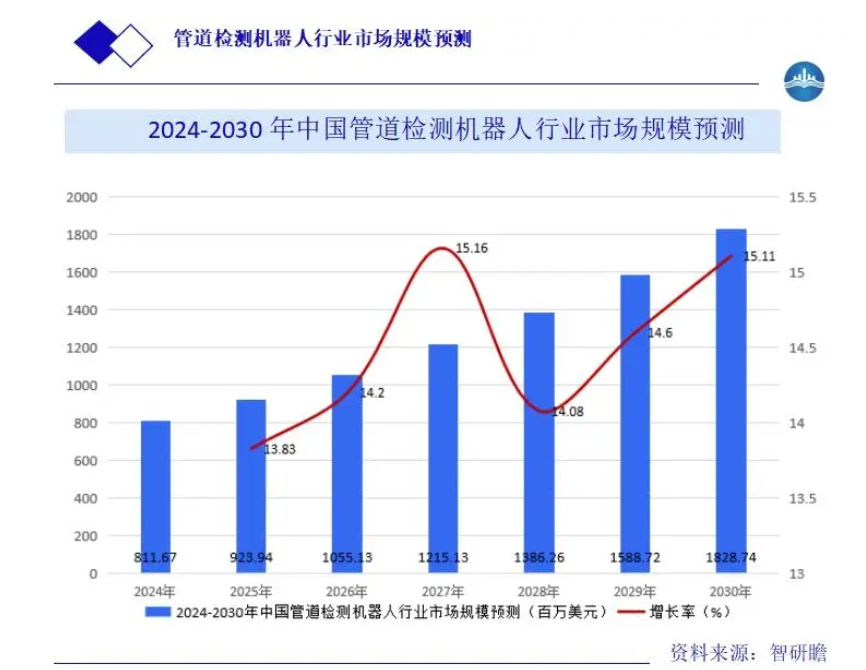
\includegraphics[width=0.55\textwidth]{7.png}
\end{itemize}






\begin{table}[htbp]
    \subsection{SWOT分析}
\centering
\caption{项目SWOT分析}
\begin{tabular}{p{0.12\textwidth}p{0.8\textwidth}}
\toprule
\textbf{维度} & \textbf{具体内容} \\
\midrule
\textbf{优势（S）} & 
1. 技术整合优势：依托双机协同架构，融合磁吸式自适应机械设计、抗干扰超声波通信与高效无线充电三大核心技术，突破传统单机设备功能局限，适配复杂工业管道场景，契合行业智能化升级需求；\\
& 2. 场景适配性强：管外机器人“立体叉字伸缩结构 + 三明治夹层转动副”可适应不同管径，管内机器人“X形剪刀结构”搭载海尔贝克磁铁阵列，能应对多障碍物、多管径管道环境，覆盖化工、石油、市政污水等核心场景；\\
& 3. 服务模式灵活：兼顾设备销售与服务运营，既能满足大型企业长期治理需求，也能通过“按需服务”降低中小企业门槛，符合行业不同规模企业的差异化需求。 \\
\midrule
\textbf{劣势（W）} & 
1. 市场认知度待提升：作为创新型技术方案，“双机协同治理”模式尚未广泛普及，客户对新技术的信任建立需要时间，初期面临传统治理方案与单机设备的竞争压力；\\
& 2. 规模化成本较高：核心零部件（如海尔贝克磁铁阵列、超声波通信模块）依赖定制化生产，短期内量产规模有限，导致设备定价相对传统产品偏高，可能影响中小企业采购意愿；\\
& 3. 服务网络初期薄弱：行业内智能化设备服务商普遍存在服务网络覆盖不足的问题，本项目初期也面临跨区域客户运维响应速度慢的挑战，需逐步构建网络服务体系。 \\
\midrule
\textbf{机遇（O）} & 
1. 政策驱动红利：国家“双碳”目标与环保监管趋严，《“十四五”生态环境监测规划》等政策强制推动企业升级管道治理设备，智能化、高效化治理方案成为市场刚需，政策背书降低市场推广难度；\\
& 2. 产业升级需求：化工、石油等行业加速绿色转型，传统治理模式效率低、成本高的弊端日益凸显，企业对低成本、高效率的智能化治理方案需求迫切，市场缺口较大；\\

\midrule
\textbf{威胁（T）} & 
1. 竞品技术追赶：传统环保设备企业（如施罗德工业集团、中仪股份）与机器人企业已布局管道检测领域，可能加速模仿双机协同技术路线，引发技术同质化竞争；\\
& 2. 价格竞争压力：国内部分中小厂商以低价策略推出低端单机设备，虽然功能单一、适配性差，但可能对价格敏感的中小企业客户形成分流。 \\
\bottomrule
\end{tabular}
\end{table}




 

 \subsection{竞品分析与行业竞争格局}


\begin{table}[htbp]

\centering
\caption{竞品类型与核心特点}
当前市场上的管道治理相关产品主要分为两类，与本项目形成差异化竞争：
\begin{tabular}{p{0.2\textwidth}p{0.3\textwidth}p{0.5\textwidth}}
\toprule
\textbf{竞品类型} & \textbf{代表厂商} & \textbf{核心特点} \\
\midrule
传统环保设备企业 & 国内：施罗德工业集团、中仪股份、特瑞升科技 & 以单机管道检测设备（如内窥镜检测机器人、爬行式检测机器人）为主，侧重单一检测功能，缺乏双机协同能力；部分产品依赖有线通信或电磁通信，在金属管道内抗干扰性弱；充电方式多为有线，续航能力有限； \\
& 国际：Honeybee Robotics、Pure Technologies & \\
传统治理服务商 & 各类环保工程公司、市政工程企业 & 以人工开挖、定点修复为核心服务，搭配基础检测设备，治理效率低、成本高、安全风险大，难以满足企业全周期管控需求。 \\
\bottomrule
\end{tabular}
\end{table}
\subsubsection{主流竞品对比}
\begin{table}[H]
\centering
\caption{主流竞品对比}
\begin{tabularx}{\linewidth}{>{\bfseries}lXXX}
\toprule
对比维度 & Honeybee Robotics（美国） & 施罗德工业集团（中国） & 中仪股份（中国）\\
\midrule
核心技术 & 单机检测 + 电磁通信 + 有线充电 & 单机检测 + 蓝牙通信 + 有线充电 & 单机检测 + 射频通信 + 有线充电\\
适配管径 & 100–1000 mm & 80–600 mm & 60–800 mm\\
越障能力 & ≤40 mm & ≤30 mm & ≤35 mm\\
通信误码率 & \textless 0.03\% & \textless 0.05\% & \textless 0.04\%\\
充电效率 & 35\%（有线） & 30\%（有线） & 32\%（有线）\\
续航能力 & 8 km（满电） & 6 km（满电） & 7 km（满电）\\
单价区间 & 120–200 万元/套 & 50–80 万元/套 & 45–90 万元/套\\
市场份额 & 12\%（2024） & 15\%（2024） & 10\%（2024）\\
核心优势 & 品牌力强、技术成熟 & 渠道广、服务响应快 & 价格低、适配场景广\\
核心劣势 & 价格高、充电方式不便 & 技术迭代慢、无无线充电 & 通信稳定性弱、续航短\\
\bottomrule
\end{tabularx}
\end{table}

\subsubsection{项目差异化优势}

\begin{enumerate}
    \item 技术路线差异化：从“单机检测”升级为“双机协同治理”，管内管外机器人配合实现全管道无盲区检测，解决传统单机设备检测盲区问题；
    \item 通信技术差异化：采用超声波通信替代电磁通信，搭配Gold序列扩频、积分滤波技术，突破金属管道电磁屏蔽与干扰难题，通信稳定性远超竞品；
    \item 续航能力差异化：搭载高效无线充电模块，40秒即可将3S锂电池从零充至满电，满电后管外机器人续航提升至10km，解决传统设备续航短、频繁充电的痛点；
    \item 服务模式差异化：从“单一设备销售”转向“设备 + 运维 + 数据”全链条服务，而非单一产品销售，增强客户粘性，抵御竞品价格竞争。
\end{enumerate}

\subsubsection{核心竞争壁垒}

\begin{enumerate}
    \item 技术壁垒：双机协同通信协议、自锁式磁吸机构、超声波抗干扰通信算法等核心技术已形成专利保护（如香港科技大学（广州）相关专利CN202510438431.4、中广核研究院专利CN202110672916.1），难以被快速复制；
    \item 场景壁垒：通过适配不同管径、不同障碍物环境的机械设计，覆盖化工、石油、市政污水等多场景，新进入者需长期积累场景数据与适配经验，门槛较高；
    \item 政策适配壁垒：产品设计严格遵循《无线充电（电力传输）设备无线电管理暂行规定》《工业固体废物污染环境防治法》等政策要求，通过政策合规性构建竞争壁垒。
\end{enumerate}

\section{商业模式}

\subsection{盈利模式}

以“短期设备销售破局，中期服务运营稳流，长期数据增值拓界”为核心逻辑，构建贴合行业现状与客户需求的盈利模式，既契合当前企业对智能化设备的采购需求，也顺应行业从“设备采购”向“服务外包”“数据赋能”的转型趋势。

\textbf{1. 设备销售：覆盖差异化客户需求，作为短期核心盈利来源，针对行业内不同规模企业的预算与场景需求，提供“基础版 + 定制版”两类产品组合：}

\begin{itemize}
    \item 基础版：包含管内管外双机协同核心模块、基础检测功能与超声波通信模块，适配中小型化工企业、县级污水处理厂等预算有限、管道场景相对简单的客户，降低初始采购门槛；
    \item 定制版：在基础版基础上，增加定制化检测模型（如化工介质腐蚀检测、石油管道压力监测）、无线充电基站、数据对接接口等，满足大型石化企业、省级化工园区等复杂管道网络与高端治理需求。
\end{itemize}

\textbf{2. 服务运营：依托设备销售积累的客户资源，打造长期盈利引擎，契合行业“轻资产运营”的趋势：}

\begin{itemize}
    \item 按场景收费服务：针对无设备采购计划的中小企业或短期治理需求客户，提供管道检测、泄漏定位、污染溯源等按次或按里程收费的服务，如全年泄漏巡检、季度管道健康检测等，解决客户“一次性投入高、使用频率低”的痛点；
    \item 年度运维服务：为已购设备客户提供定期保养、模块升级、技术支持等运维服务，包括设备校准、软件迭代、零部件更换等，延长设备使用寿命，提升客户使用体验。此类服务可形成稳定现金流，增强客户粘性，行业内同类运维服务毛利率普遍达60\%以上。
\end{itemize}

\textbf{3. 数据增值：随着管道治理智能化水平提升，数据成为核心生产要素，数据增值服务是行业未来重要盈利方向：}

\begin{itemize}
    \item 企业级数据服务：为客户提供管道健康档案管理、风险预警、维护方案优化等服务，基于机器人检测数据生成个性化报告，助力企业实现精细化环境管控；
    \item 公共部门数据服务：为环保部门、园区管委会提供区域污染分布分析、行业治理趋势研判等决策支持服务，通过长期订阅模式拓展收益边界。此类服务既符合环保监管部门的数字化监管需求，也能提升项目的社会价值与政策适配性。
\end{itemize}

\begin{figure}[htbp]
    \centering
    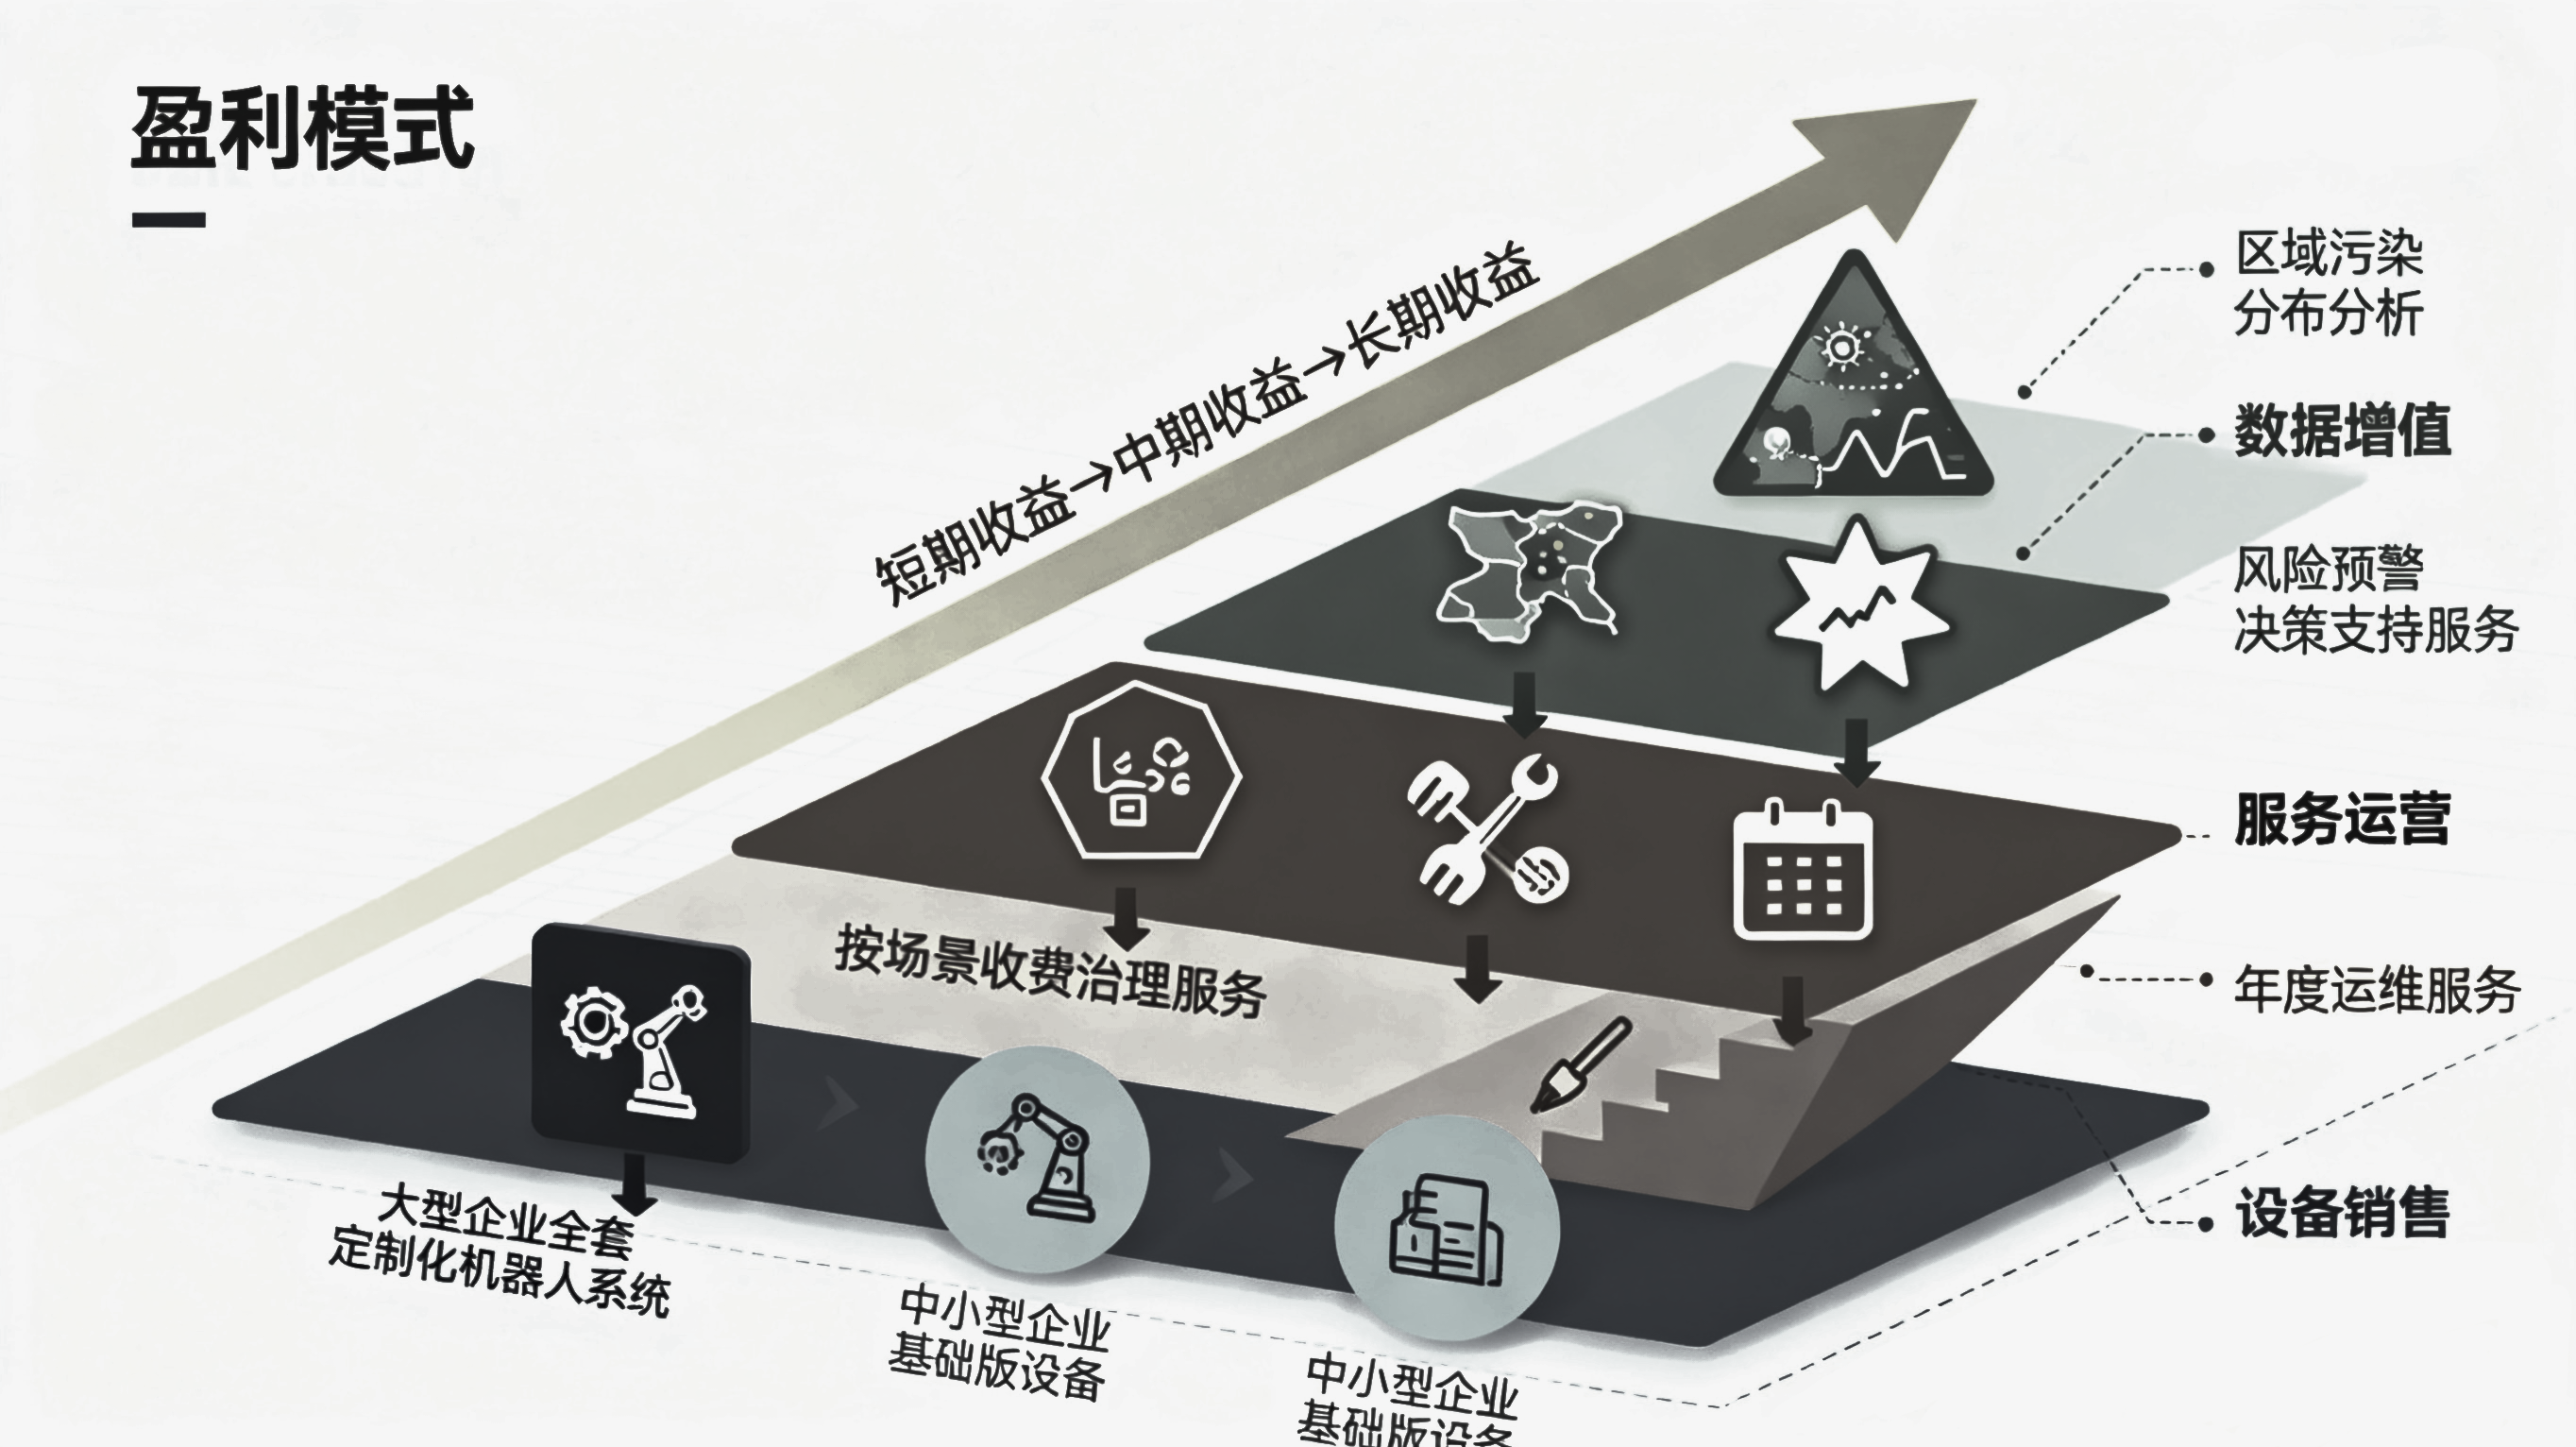
\includegraphics[width=0.85\textwidth]{6.png}
    \caption{盈利模式}
\end{figure}

\subsection{渠道策略}

围绕工业管道环境治理的核心场景，构建“直接销售 + 合作伙伴”的双渠道体系，确保快速触达目标客户，契合行业客户集中、决策链长的特点：

\textbf{1. 直接销售渠道：}

\begin{itemize}
    \item 组建行业专项销售团队：组建化工、石油、市政污水三大行业专项销售团队，重点覆盖长三角、珠三角、环渤海等核心产业聚集区。通过一对一沟通，深入了解客户管道布局、治理痛点与预算需求，提供定制化解决方案，匹配行业大客户决策流程长、需求个性化的特点；
    \item 行业展会与论坛：参与中国国际环保展览会、中国化工园区发展大会、石油化工行业设备展等顶级行业展会，以及地方环保部门组织的政策宣贯会，展示产品技术优势与行业应用案例，增强客户信任。行业展会是环保设备企业获取客户资源的核心渠道，转化率高；
    \item 线上精准营销：搭建官网、微信公众号等数字化平台，发布行业政策解读、管道治理痛点分析、产品技术原理等内容，吸引潜在客户咨询，同时通过行业垂直媒体投放广告，实现精准触达。
\end{itemize}

\textbf{2. 合作伙伴渠道：}

\begin{itemize}
    \item 环保工程公司合作：与国内头部环保工程公司建立深度合作，将双机协同机器人系统融入其整体环保服务方案。环保工程公司具备丰富的项目资源与客户基础，可快速将产品导入化工园区、市政污水治理等项目场景；
    \item 园区运营方合作：与省级以上化工园区、石油炼化基地运营方签订合作协议，成为园区指定管道治理设备供应商或服务提供商。园区内企业集中，管道治理需求统一，可实现批量销售与服务；
    \item 政府渠道联动：与地方环保部门建立合作关系，参与区域环境治理项目、管网更新改造工程等政府主导项目，依托政策背书提升品牌影响力与市场渗透率。政府项目具有示范效应，可带动周边企业采购。
\end{itemize}

\subsection{客户服务}

针对行业内不同类型客户的需求特点，制定专属服务策略，契合大型企业、中小企业与公共部门的差异化需求：

\textbf{1. 大型企业客户：提供定制化全流程服务}

\begin{itemize}
    \item 方案定制：结合企业管道网络规模、介质类型、治理标准，设计全流程治理方案，包括设备部署、检测流程、数据对接等；
    \item 数字化对接：将机器人系统检测数据与企业环保管理平台打通，实现实时监控、数据互通与报表自动生成，助力企业提升管理效率；
    \item 专属服务团队：配备1名专属顾问 + 2名技术工程师，提供7×24小时响应服务，定期上门巡检设备运行状态，确保设备稳定运行。
\end{itemize}

\textbf{2. 中小型企业客户：提供轻量化低成本服务}

\begin{itemize}
    \item 简化操作流程：优化设备操作界面，提供线上视频培训与图文手册，降低操作人员学习成本；
    \item 灵活合作模式：推出“以租代购”“按需付费”等模式，降低客户一次性资金压力，契合中小企业预算有限的特点；
    \item 快速响应服务：建立5×8小时响应机制，通过远程指导解决常见问题，对于复杂故障提供上门服务，平衡服务质量与成本。
\end{itemize}

\textbf{3. 公共部门客户：提供专业化监管支撑服务}

\begin{itemize}
    \item 区域协同调度：提供多机器人协同调度服务，满足大面积、多管线的管道治理需求，适配环保部门区域监管职责；
    \item 标准化报告输出：按照政策要求生成标准化污染治理报告、管道健康评估报告，为环保监管提供数据依据；
    \item 政策合规支持：提供政策解读服务，协助公共部门客户落实环保监管要求，确保治理工作符合政策标准。
\end{itemize}

\begin{figure}[htbp]
    \centering
    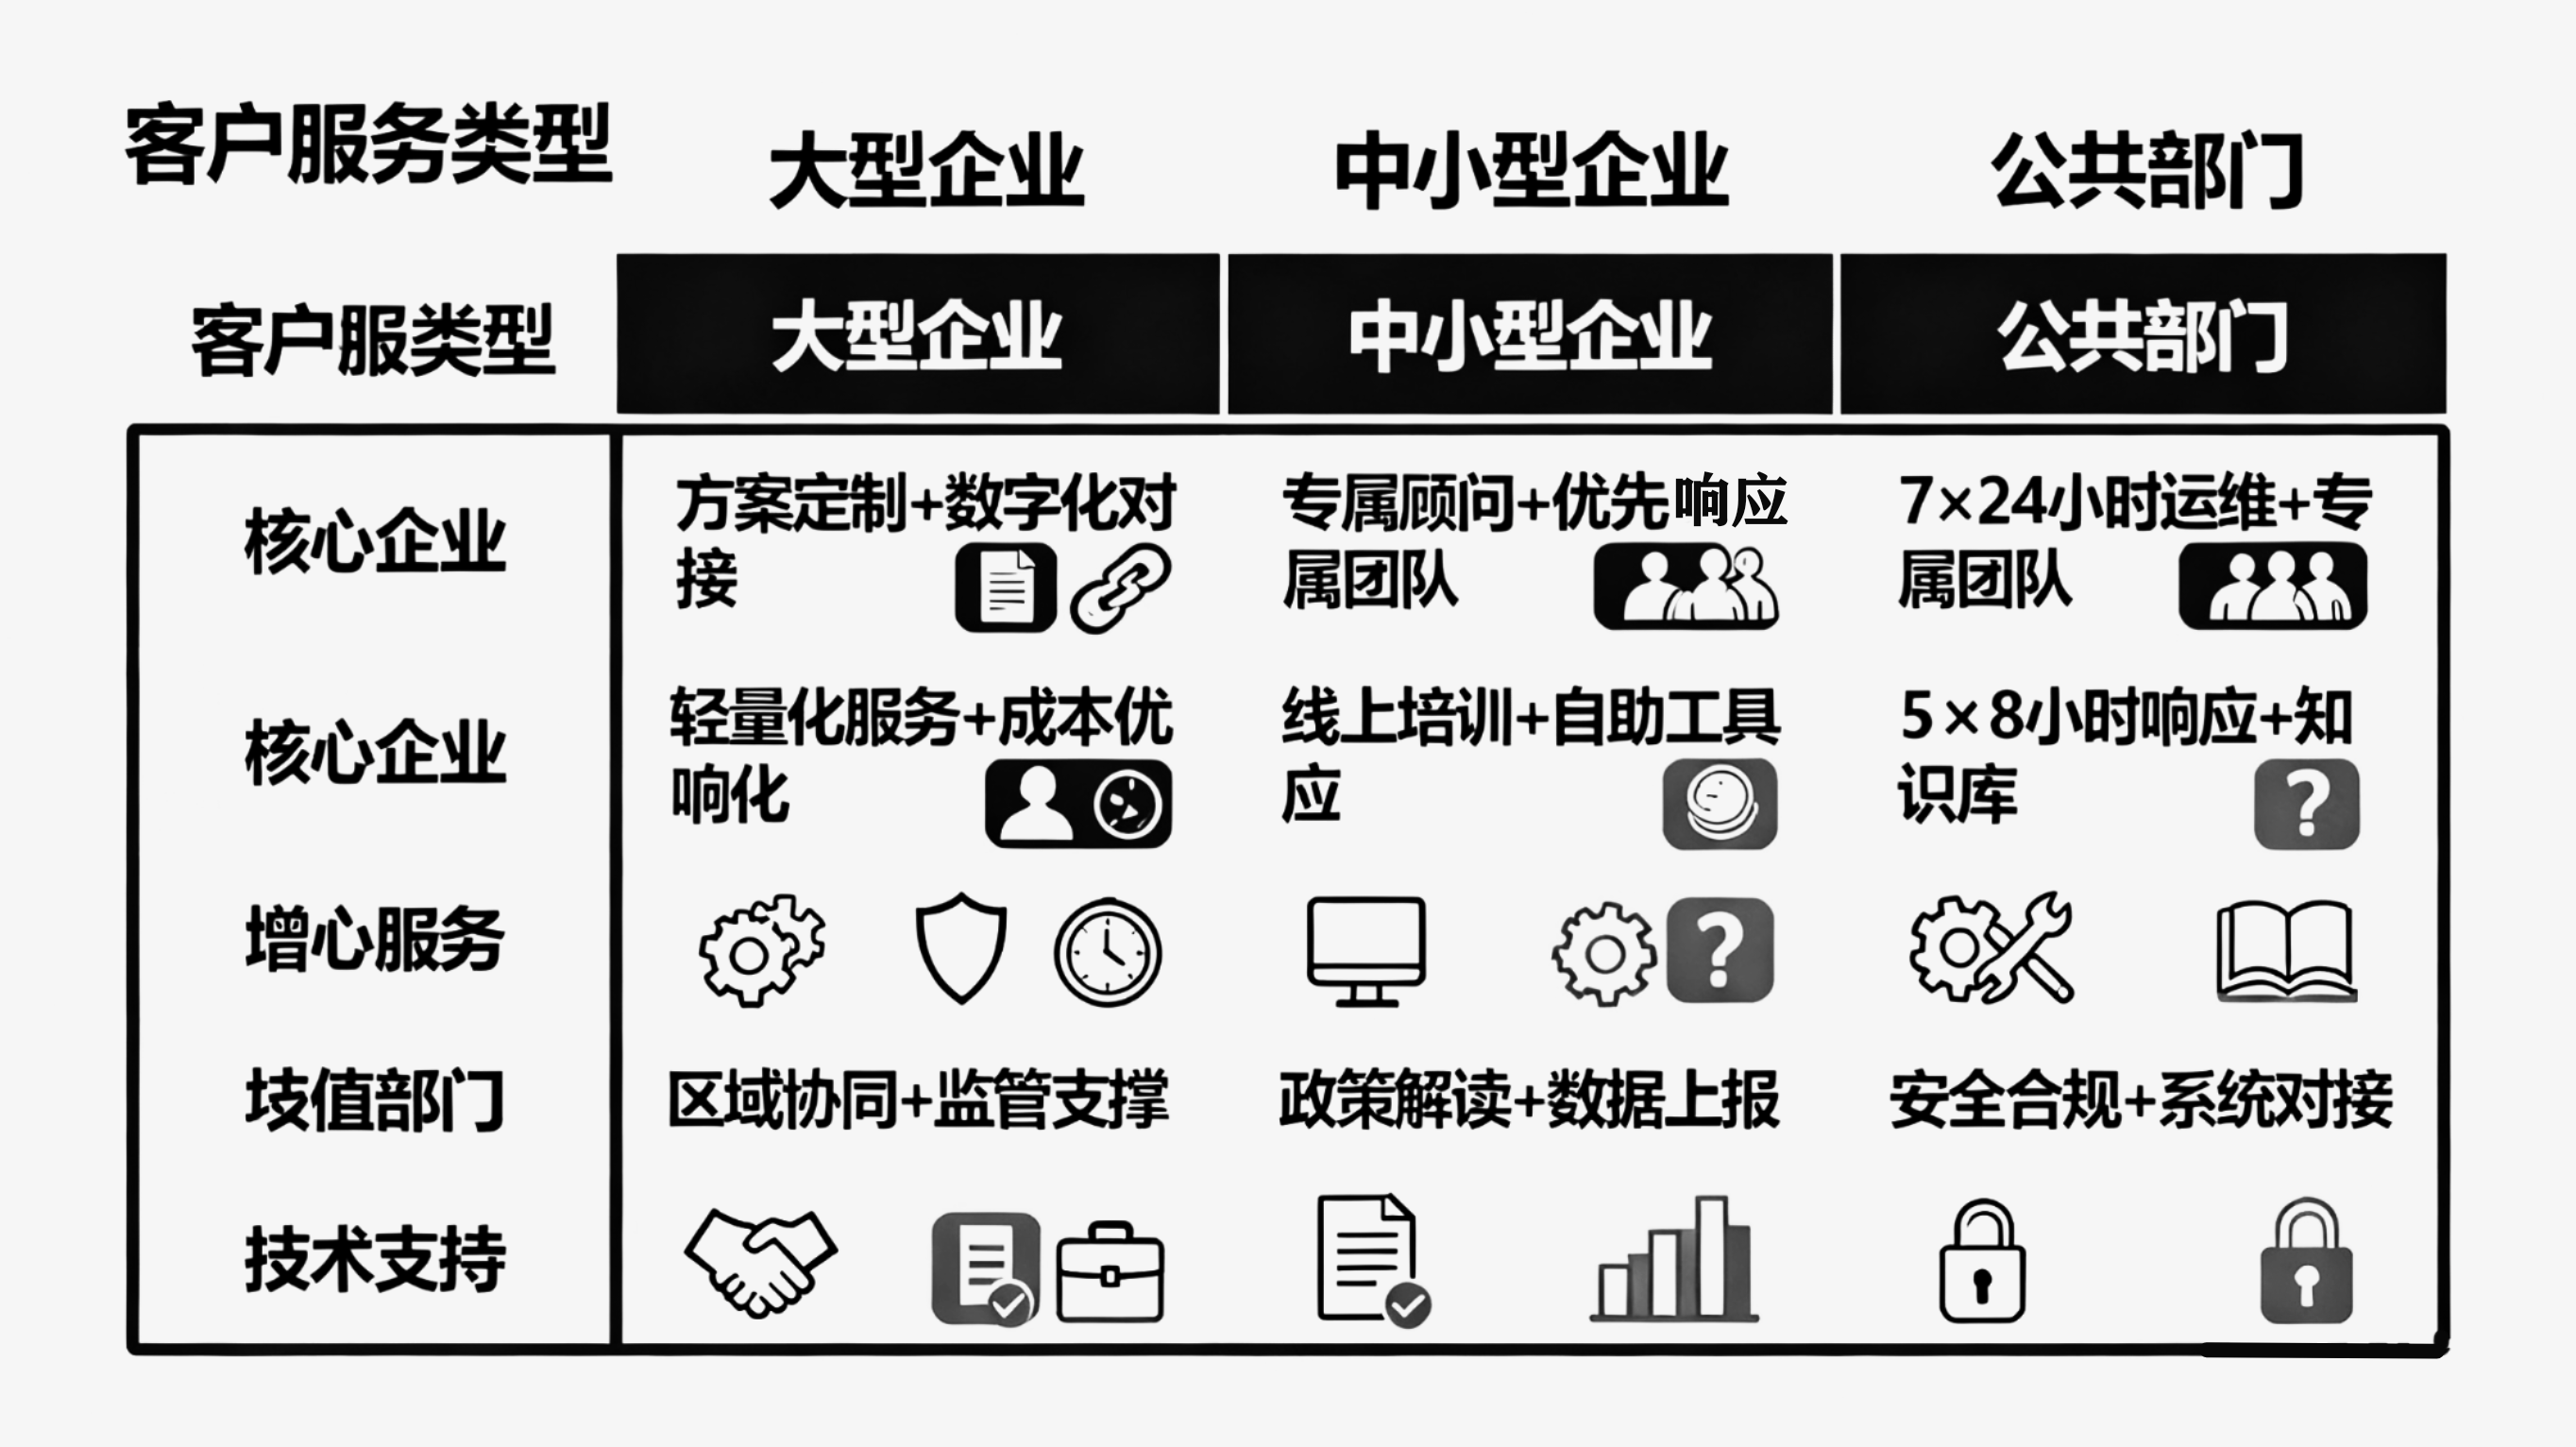
\includegraphics[width=0.75\textwidth]{5.png}
    \caption{客户服务}
\end{figure}

\section{结论}

双机协同管道环境治理机器人项目，精准契合国家“双碳”目标与环保监管趋严的政策导向，聚焦工业管道泄漏、堵塞及内壁污染等核心痛点，通过创新技术构建差异化竞争优势。其以管内管外双机协同为核心架构，融合磁吸式自适应机械设计、抗干扰超声波通信与高效无线充电三大关键技术，突破传统人工治理效率低、安全风险高、存在检测盲区的局限，可灵活适配化工、石油、市政污水等多场景复杂管道环境。

从市场潜力看，国内工业管道环境治理市场规模增长迅猛，2028年将突破1800亿元，智能化设备占比持续提升，项目既具备短期设备销售的盈利支撑，又可通过长期服务运营与数据增值拓展收益空间，整体兼具技术可行性与商业价值，发展前景广阔。

\newpage
\section{References }

\begin{enumerate}
    \item JICHUN XING, CHAO NING, YINGXIANG LIU, et al. Piezoelectric inertial robot for operating in small pipelines based on stick-slip mechanism: modeling and experiment[J]. \textit{Frontiers of Mechanical Engineering}, 2022, 17(3): 41.
    \item 李孟春, 武利生, 郑利红, 等. 电磁驱动的小型管道机器人研究[J]. \textit{太原理工大学学报}, 2002, 33(2): 189-191,200.
    \item 香港科技大学(广州). 管道机器人: CN202510438431.4[P]. 2025-07-04.
    \item 中广核研究院有限公司, 中国广核集团有限公司, 中国广核电力股份有限公司. 管道机器人: CN202110672916.1[P]. 2023-03-24.
    \item 内蒙古科技大学. 一种智能自适应管道机器人: CN202422141315.X[P]. 2025-07-11.
    \item 徐洪涛. 油气管道牵引机器人设计与仿真[J]. \textit{管道技术与设备}, 2021(1): 37-41.
    \item 国家能源局. 国家能源局关于加快推进能源数字化智能化发展的若干意见（国能发科技〔2023〕27号）[EB/OL]. 2023-03-28.
    \item 北京博研智尚信息咨询有限公司. 2025年中国管网机器人行业市场前景预测及投资价值评估分析报告[R]. 2025.
    \item 中华人民共和国生态环境部. 2023中国生态环境状况公报[EB/OL]. 2024-06-05.
    \item 中华人民共和国生态环境部. 入河排污口监督管理办法（生态环境部令第35号）[EB/OL]. 2024-11-01.
    \item 中国城镇供水排水协会. 2024年中国城镇污水管网发展报告[R]. 2024.
    \item 头豹研究院. 2024年全球管道检测机器人行业白皮书[R]. 2024.
    \item 艾瑞咨询. 2023年中国工业管道治理行业白皮书[R]. 2023.
    \item 中仪股份. 2023年年度报告[R]. 2024.
    \item 江苏省生态环境厅. 江苏省化工园区智能化改造专项补贴政策（苏环办〔2024〕12号）[EB/OL]. 2024-03-15.
    \item 中国化工园区协会. 2024年中国化工园区发展报告[R]. 2024.
    \item 双机协同管道环境治理机器人项目团队. 项目技术手册、财务规划、营销规划等内部报告[R]. 2025.
    \item 施罗德工业集团. 2023年年度报告[R]. 2024.
    \item 国家统计局. 2024年中国工业企业环保投入统计公报[EB/OL]. 2024-08-20.
    \item 中国机械工业联合会. 2024年中国智能装备行业发展报告[R]. 2024.
    \item 中华人民共和国生态环境部. 2024年区域生态环境质量报告[EB/OL]. 2024-09-10.
    \item 国家无线电管理局. 无线充电（电力传输）设备无线电管理暂行规定[EB/OL]. 2024-01-05.
\end{enumerate}

\end{document}












